% ============================================================
%  Network Security -- Module 3: Security Goals, Authorization and Access Control
%  Lesson 4: Security and Authorization
%  Lesson 7: Multi Level Model of Security
%  Beamer (Madrid theme). Compile with: pdflatex module3.tex (twice)
% ============================================================
\documentclass[aspectratio=169,11pt,xcolor={table}]{beamer}
\usetheme{Madrid}
\usefonttheme{professionalfonts}

\usepackage[T1]{fontenc}
\usepackage{lmodern}
\usepackage{booktabs}
\usepackage{array}
\usepackage{tikz}
\usetikzlibrary{arrows.meta,positioning,shapes.geometric,shapes.symbols,
  shapes.misc,shadows,calc,fit,backgrounds,mindmap,decorations.pathmorphing,decorations.pathreplacing}

% ------------------------------------------------------------
%  Colour palette
% ------------------------------------------------------------
\definecolor{navy}{RGB}{21,45,99}
\definecolor{ocean}{RGB}{28,97,158}
\definecolor{aqua}{RGB}{0,142,150}
\definecolor{brick}{RGB}{200,55,45}
\definecolor{amber}{RGB}{235,150,20}
\definecolor{leaf}{RGB}{40,160,90}
\definecolor{grape}{RGB}{125,70,165}
\definecolor{sky}{RGB}{235,243,252}
\definecolor{ink}{RGB}{40,40,50}

\setbeamercolor{palette primary}{bg=ocean,fg=white}
\setbeamercolor{palette secondary}{bg=navy!85,fg=white}
\setbeamercolor{palette tertiary}{bg=navy,fg=white}
\setbeamercolor{palette quaternary}{bg=navy,fg=white}
\setbeamercolor{structure}{fg=ocean}
\setbeamercolor{title}{bg=navy,fg=white}
\setbeamercolor{frametitle}{bg=navy,fg=white}
\setbeamercolor{block title}{bg=ocean,fg=white}
\setbeamercolor{block body}{bg=sky,fg=ink}
\setbeamercolor{block title alerted}{bg=brick,fg=white}
\setbeamercolor{block body alerted}{bg=brick!8,fg=ink}
\setbeamercolor{block title example}{bg=leaf,fg=white}
\setbeamercolor{block body example}{bg=leaf!8,fg=ink}
\setbeamercolor{normal text}{fg=ink}
\setbeamercolor{alerted text}{fg=brick}
\setbeamercolor{item projected}{bg=ocean,fg=white}
\setbeamertemplate{items}[circle]
\setbeamertemplate{blocks}[rounded][shadow=true]
\setbeamertemplate{navigation symbols}{}

% Section divider slide
\AtBeginSection[]{
  \begin{frame}[plain]
    \begin{tikzpicture}[remember picture,overlay]
      \fill[navy] (current page.south west) rectangle (current page.north east);
      \fill[ocean] (current page.south west) rectangle ([yshift=1.2cm]current page.south east);
      \fill[aqua] ([yshift=1.2cm]current page.south west) rectangle ([yshift=1.35cm]current page.south east);
      \foreach \i in {1,...,6}
        \draw[white,opacity=0.06,line width=14pt]
          ([xshift=\i*1.6cm]current page.north west) circle (\i*0.9cm);
      \node[white,font=\large,anchor=west] at ([xshift=1.2cm,yshift=0.9cm]current page.west)
        {Lesson \thesection};
      \node[white,font=\huge\bfseries,anchor=west,text width=12cm] at ([xshift=1.2cm,yshift=-0.1cm]current page.west)
        {\insertsectionhead};
      \node[white,opacity=0.8,anchor=east,font=\small] at ([xshift=-0.8cm,yshift=0.6cm]current page.south east)
        {Module 3 \,$\cdot$\, Security Goals, Authorization and Access Control};
    \end{tikzpicture}
  \end{frame}
}

% ------------------------------------------------------------
%  TikZ styles and small pictograms
% ------------------------------------------------------------
\tikzset{
  >={Stealth[length=2.6mm]},
  box/.style={draw=#1!80!black,fill=#1!15,rounded corners=4pt,thick,
    minimum height=8mm,minimum width=22mm,align=center,font=\small,
    drop shadow={opacity=0.25}},
  box/.default=ocean,
  lay/.style={fill=#1,text=white,rounded corners=3pt,minimum width=38mm,minimum height=9mm,font=\scriptsize,align=center},
  solid box/.style={fill=#1,text=white,rounded corners=4pt,
    minimum height=8mm,minimum width=22mm,align=center,font=\small\bfseries,
    drop shadow={opacity=0.3}},
  solid box/.default=ocean,
  flow/.style={->,very thick,draw=#1},
  flow/.default=ink!70,
  station/.style={circle,draw=#1!80!black,fill=#1!20,very thick,minimum size=13mm,
    font=\small\bfseries,align=center},
  station/.default=ocean,
  tag/.style={font=\scriptsize,text=ink!80,align=center},
  layer/.style={draw=white,thick,fill=#1,text=white,minimum width=40mm,
    minimum height=6.5mm,font=\small\bfseries},
  % pictograms
  pics/pc/.style={code={
    \fill[#1!85!black,rounded corners=1.5pt] (-0.42,-0.05) rectangle (0.42,0.52);
    \fill[white!90!#1] (-0.36,0.01) rectangle (0.36,0.46);
    \fill[#1!85!black] (-0.06,-0.05) rectangle (0.06,-0.18);
    \fill[#1!85!black,rounded corners=1pt] (-0.24,-0.18) rectangle (0.24,-0.24);
  }},
  pics/pc/.default=ocean,
  pics/person/.style={code={
    \fill[#1] (0,0.46) circle (0.16);
    \fill[#1,rounded corners=5pt] (-0.27,-0.1) -- (-0.27,0.2) -- (0.27,0.2) -- (0.27,-0.1) -- cycle;
  }},
  pics/person/.default=ocean,
  pics/lock/.style={code={
    \draw[#1!80!black,line width=2.2pt] (-0.15,0.12) -- (-0.15,0.28) arc (180:0:0.15) -- (0.15,0.12);
    \fill[#1,rounded corners=2pt] (-0.26,-0.22) rectangle (0.26,0.14);
    \fill[white] (0,-0.02) circle (0.05);
    \fill[white] (-0.02,-0.02) rectangle (0.02,-0.13);
  }},
  pics/lock/.default=amber,
  pics/doc/.style={code={
    \fill[white,draw=#1,thick] (-0.25,-0.33) -- (-0.25,0.33) -- (0.12,0.33) -- (0.25,0.2) -- (0.25,-0.33) -- cycle;
    \draw[#1,thick] (0.12,0.33) -- (0.12,0.2) -- (0.25,0.2);
    \foreach \y in {0.12,0,-0.12,-0.24} \draw[#1!70,thick] (-0.16,\y) -- (0.16,\y);
  }},
  pics/doc/.default=ocean,
  pics/key/.style={code={
    \draw[#1,line width=2pt] (0,0) circle (0.12);
    \draw[#1,line width=2pt] (0.12,0) -- (0.5,0) (0.38,0) -- (0.38,-0.12) (0.47,0) -- (0.47,-0.1);
  }},
  pics/key/.default=amber,
}
\newcommand{\comma}{,}
\newcommand{\hl}[1]{\textcolor{ocean}{\textbf{#1}}}
\newcommand{\bad}[1]{\textcolor{brick}{\textbf{#1}}}
\newcommand{\good}[1]{\textcolor{leaf}{\textbf{#1}}}

\makeatletter
% University logo, small, top-right corner of every page
\AddToHook{shipout/foreground}{%
  \put(\strip@pt\paperwidth,0){%
    \makebox(0,0)[tr]{\raisebox{-0.8cm}{
\includegraphics[height=0.72cm]{au_logo.png}\hspace{0.15cm}}}}}
\makeatother

% ------------------------------------------------------------
\title[Module 3: Goals \& Access Control]{Security Goals, Authorization and Access Control}
\subtitle{Module 3 \,\textbar\, Lesson 4: Security and Authorization \,\textbullet\, Lesson 7: Multi Level Model of Security}
\author[Network Security]{Network Security}
\institute[SLM]{Self-Learning Material \,--\, Lessons 4 \& 7}
\date{}

\begin{document}

% ============================================================
\begin{frame}[plain]
  
\begin{tikzpicture}[remember picture,overlay]
    \shade[top color=navy,bottom color=ocean] (current page.south west) rectangle (current page.north east);
    \foreach \i/\o in {1/0.10,2/0.08,3/0.06,4/0.05,5/0.04}
      \draw[white,opacity=\o,line width=1.2pt] ([xshift=-2.5cm,yshift=-0.5cm]current page.north east) circle (\i*1.1cm);
    \fill[aqua] ([yshift=2.35cm]current page.south west) rectangle ([yshift=2.45cm]current page.south east);
    % motif: layered rings (multi-level security) around a key
    \begin{scope}[shift={([xshift=-2.4cm,yshift=0.2cm]current page.east)},scale=0.85]
      \foreach \r/\o in {1.9/0.15,1.45/0.25,1.0/0.4}
        \fill[white,opacity=\o] (0,0) circle (\r);
      \node[circle,fill=amber,minimum size=12mm] at (0,0) {};
      \pic[scale=1.3] at (-0.22,0) {key=white};
      \foreach \a in {30,150,270} \pic[scale=0.45] at (\a:1.68) {person=white};
    \end{scope}
    \node[white,anchor=west,font=\normalsize] at ([xshift=1.1cm,yshift=2.4cm]current page.west)
      {NETWORK SECURITY \,\textbar\, MODULE 3};
    \node[white,anchor=west,font=\fontsize{21}{26}\selectfont\bfseries,text width=10.5cm] at ([xshift=1.1cm,yshift=1.0cm]current page.west)
      {Security Goals, Authorization\\[2pt] and Access Control};
    \node[white,opacity=0.9,anchor=west,text width=9cm,font=\small] at ([xshift=1.1cm,yshift=-0.9cm]current page.west)
      {Lesson 4 \,--\, Security and Authorization\\ Lesson 7 \,--\, Multi Level Model of Security};
    \node[white,opacity=0.85,anchor=west,font=\footnotesize] at ([xshift=1.1cm,yshift=1.2cm]current page.south west)
      {CIA \,$\cdot$\, Risk analysis \,$\cdot$\, Threats \& vulnerabilities \,$\cdot$\, Authentication \,$\cdot$\, Passwords \,$\cdot$\, Firewalls \,$\cdot$\, IDS \,$\cdot$\, Auditing};
  \end{tikzpicture}
\end{frame}

% ============================================================
\begin{frame}{Roadmap of This Module}
  \centering
  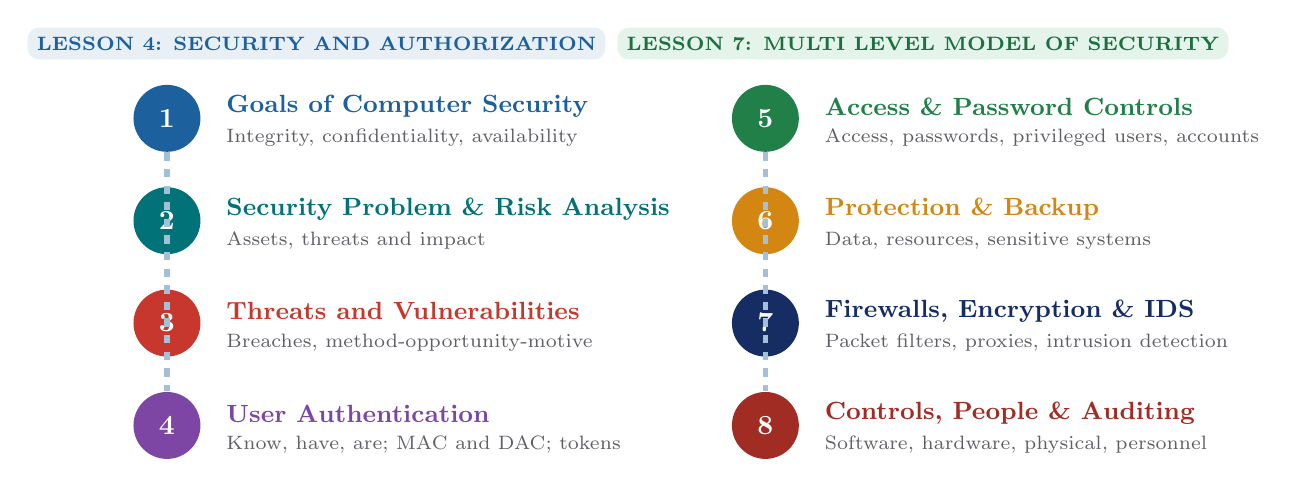
\begin{tikzpicture}
    \foreach \t/\c/\n [count=\i] in {
      Goals of Computer Security/ocean/Integrity\comma{} confidentiality\comma{} availability,
      Security Problem \& Risk Analysis/aqua!80!black/Assets\comma{} threats and impact,
      Threats and Vulnerabilities/brick/Breaches\comma{} method-opportunity-motive,
      User Authentication/grape/Know\comma{} have\comma{} are; MAC and DAC; tokens,
      Access \& Password Controls/leaf!80!black/Access\comma{} passwords\comma{} privileged users\comma{} accounts,
      Protection \& Backup/amber!90!black/Data\comma{} resources\comma{} sensitive systems,
      Firewalls\comma{} Encryption \& IDS/navy/Packet filters\comma{} proxies\comma{} intrusion detection,
      Controls\comma{} People \& Auditing/brick!80!black/Software\comma{} hardware\comma{} physical\comma{} personnel}
    {
      \pgfmathsetmacro{\x}{ifthenelse(\i<5,0,7.6)}
      \pgfmathsetmacro{\y}{-mod(\i-1,4)*1.3}
      \node[circle,fill=\c,text=white,font=\bfseries,minimum size=8.5mm] (n\i) at (\x,\y) {\i};
      \node[anchor=west,font=\small\bfseries,text=\c] at ([xshift=2mm,yshift=1.5mm]n\i.east) {\t};
      \node[anchor=west,font=\scriptsize,text=ink!75] at ([xshift=2mm,yshift=-2.5mm]n\i.east) {\n};
    }
    \draw[ocean!40,line width=2pt,dashed] (n1) -- (n4);
    \draw[ocean!40,line width=2pt,dashed] (n5) -- (n8);
    \node[fill=ocean!10,rounded corners,font=\scriptsize\bfseries,text=ocean] at (1.9,0.95) {LESSON 4: SECURITY AND AUTHORIZATION};
    \node[fill=leaf!12,rounded corners,font=\scriptsize\bfseries,text=leaf!70!black] at (9.6,0.95) {LESSON 7: MULTI LEVEL MODEL OF SECURITY};
  \end{tikzpicture}
\end{frame}

% ============================================================
\setcounter{section}{3}
\section{Security and Authorization}
% ============================================================

\begin{frame}{What You Will Learn in Lesson 4}
  \begin{columns}[c]
    \begin{column}{0.5\textwidth}
      \centering
      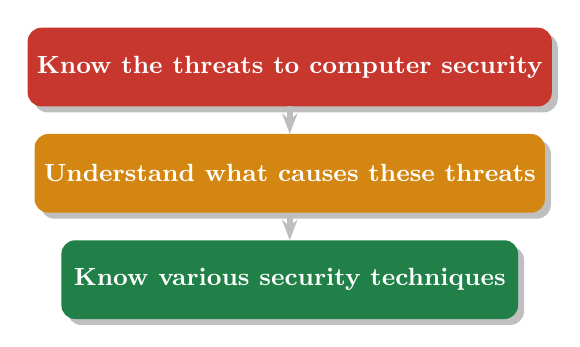
\begin{tikzpicture}
        \foreach \t/\c/\y in {Know the threats to computer security/brick/0,Understand what causes these threats/amber!90!black/-1.35,Know various security techniques/leaf!80!black/-2.7}{
          \node[fill=\c,text=white,rounded corners=5pt,minimum width=58mm,minimum height=10mm,font=\small\bfseries,drop shadow] at (0,\y) {\t};
        }
        \draw[->,line width=2pt,ink!30] (0,-0.5) -- (0,-0.85);
        \draw[->,line width=2pt,ink!30] (0,-1.85) -- (0,-2.2);
      \end{tikzpicture}
    \end{column}
    \begin{column}{0.48\textwidth}
      \begin{block}{The big question}
        \small How do we decide \textbf{what} to protect, \textbf{from whom}, and \textbf{how}, and then make sure only the \textbf{right people} get in?
      \end{block}
      \vspace{2mm}
      \begin{itemize}\small\setlength{\itemsep}{3pt}
        \item Goals: \textbf{C}, \textbf{I}, \textbf{A}
        \item Risk analysis in 3 steps
        \item Threats vs.\ vulnerabilities
        \item Authentication and authorization
      \end{itemize}
    \end{column}
  \end{columns}
\end{frame}

% ------------------------------------------------------------
\begin{frame}{Goals of Computer Security}
  \begin{columns}[c]
    \begin{column}{0.5\textwidth}
      \centering
      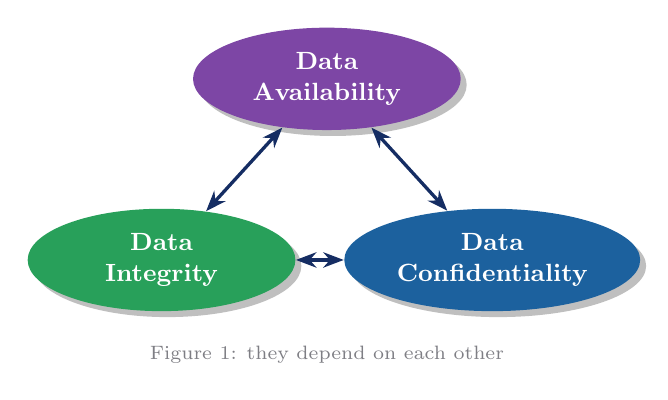
\begin{tikzpicture}
        \node[ellipse,fill=grape,text=white,font=\small\bfseries,minimum width=34mm,minimum height=13mm,align=center,drop shadow] (a) at (0,1.6) {Data\\Availability};
        \node[ellipse,fill=leaf,text=white,font=\small\bfseries,minimum width=34mm,minimum height=13mm,align=center,drop shadow] (i) at (-2.1,-0.7) {Data\\Integrity};
        \node[ellipse,fill=ocean,text=white,font=\small\bfseries,minimum width=34mm,minimum height=13mm,align=center,drop shadow] (c) at (2.1,-0.7) {Data\\Confidentiality};
        \draw[<->,very thick,navy] (a) -- (i); \draw[<->,very thick,navy] (a) -- (c); \draw[<->,very thick,navy] (i) -- (c);
        \node[font=\scriptsize,text=ink!60] at (0,-1.9) {Figure 1: they depend on each other};
      \end{tikzpicture}
    \end{column}
    \begin{column}{0.48\textwidth}
      \begin{itemize}\setlength{\itemsep}{6pt}\small
        \item The goals of computer security are \textbf{integrity}, \textbf{confidentiality} and \textbf{availability} of the information managed by the system
        \item The three are \textbf{related}: improving one can weaken another
      \end{itemize}
      \vspace{2mm}
      \begin{exampleblock}{Example of the tension}
        \small Locking data away very tightly improves confidentiality, but it can \textbf{hurt availability} for the people who need it.
      \end{exampleblock}
    \end{column}
  \end{columns}
\end{frame}

% ------------------------------------------------------------
\begin{frame}{Goal 1: Integrity}
  \centering
  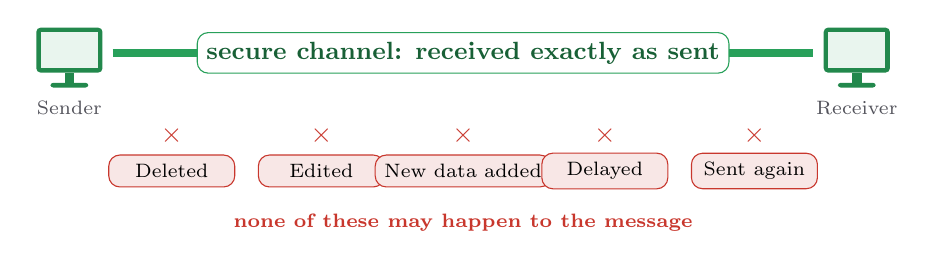
\begin{tikzpicture}
    \pic at (0,0) {pc=leaf}; \node[tag] at (0,-0.5) {Sender};
    \pic at (10,0) {pc=leaf}; \node[tag] at (10,-0.5) {Receiver};
    \draw[leaf,line width=3pt] (0.55,0.2) -- (9.45,0.2);
    \node[fill=white,draw=leaf,rounded corners,font=\small\bfseries,text=leaf!60!black] at (5,0.2) {secure channel: received exactly as sent};
    \foreach \x/\t in {1.3/Deleted,3.2/Edited,5.0/New data added,6.8/Delayed,8.7/Sent again}{
      \node[fill=brick!12,draw=brick,rounded corners,font=\scriptsize,minimum width=16mm] at (\x,-1.3) {\t};
      \node[brick,font=\bfseries] at (\x,-0.85) {$\times$};
    }
    \node[font=\scriptsize\bfseries,text=brick] at (5,-1.95) {none of these may happen to the message};
  \end{tikzpicture}
  \vspace{3mm}
  \begin{columns}[T]
    \begin{column}{0.5\textwidth}
      \begin{block}{Definition}
        \small Data sent through the secure channel is \textbf{not altered or tampered} with by others.
      \end{block}
    \end{column}
    \begin{column}{0.46\textwidth}
      \begin{alertblock}{Note}
        \small Integrity does \textbf{not} stop a third party from \emph{viewing} the data; it only guarantees nobody \emph{modified} it.
      \end{alertblock}
    \end{column}
  \end{columns}
\end{frame}

% ------------------------------------------------------------
\begin{frame}{Goal 2: Confidentiality}
  \begin{columns}[c]
    \begin{column}{0.5\textwidth}
      \centering
      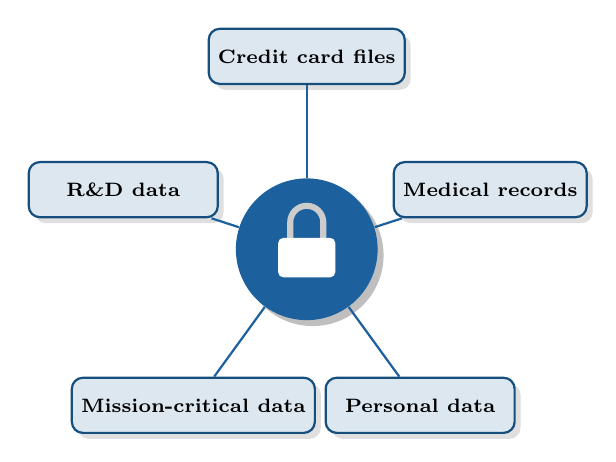
\begin{tikzpicture}
        \node[circle,fill=ocean,minimum size=18mm,drop shadow] (c) at (0,0) {};
        \pic[scale=1.4] at (0,-0.05) {lock=white};
        \foreach \a/\t in {90/Credit card files,18/Medical records,-54/Personal data,-126/Mission-critical data,162/R\&D data}{
          \node[box=ocean,minimum width=24mm,minimum height=7mm,font=\scriptsize\bfseries] (s\a) at (\a:2.45) {\t};
          \draw[ocean,thick] (c) -- (s\a);
        }
      \end{tikzpicture}
    \end{column}
    \begin{column}{0.48\textwidth}
      \begin{block}{Definition}
        \small When data travels from source to destination, \textbf{nobody except the intended person} can view it.
      \end{block}
      \begin{itemize}\small\setlength{\itemsep}{3pt}
        \item A network with no confidentiality is \textbf{not secure}
        \item Minimum requirement: the mail you send a friend is \textbf{not read by anyone else}
        \item If people cannot trust e-mail to be confidential, they \textbf{never use it}
      \end{itemize}
    \end{column}
  \end{columns}
\end{frame}

% ------------------------------------------------------------
\begin{frame}{Goal 3: Availability}
  \begin{columns}[c]
    \begin{column}{0.46\textwidth}
      \begin{block}{Definition}
        \small The system is \textbf{accessible to authorized persons at appropriate times}.
      \end{block}
      \vspace{2mm}
      \begin{alertblock}{Balance}
        \small There is no point making a system so secure that \textbf{no user can access} the data they need to do their jobs.
      \end{alertblock}
    \end{column}
    \begin{column}{0.52\textwidth}
      \centering
      \textbf{\textcolor{grape}{A computer system is available if\dots}}\\[3mm]
      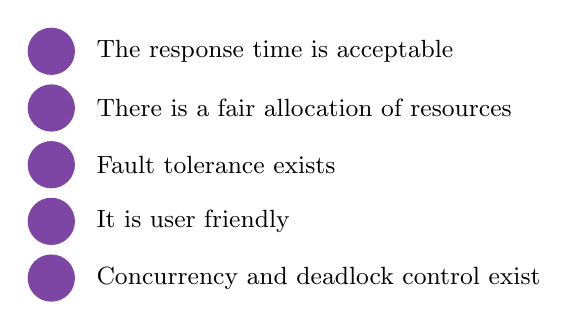
\begin{tikzpicture}
        \foreach \t [count=\i from 0] in {The response time is acceptable,There is a fair allocation of resources,Fault tolerance exists,It is user friendly,Concurrency and deadlock control exist}{
          \node[circle,fill=grape,text=white,font=\scriptsize\bfseries,minimum size=6mm] at (0,-\i*0.72) {\checkmark};
          \node[anchor=west,font=\small] at (0.45,-\i*0.72) {\t};
        }
      \end{tikzpicture}
    \end{column}
  \end{columns}
\end{frame}

% ------------------------------------------------------------
\begin{frame}{The Security Problem}
  \centering
  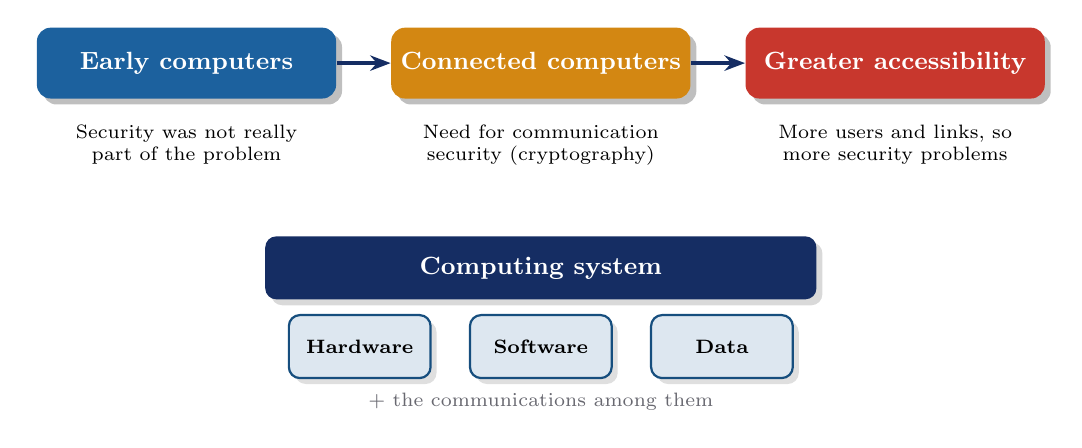
\begin{tikzpicture}
    \foreach \x/\c/\t/\d [count=\i] in {0/ocean/Early computers/Security was not really part of the problem,4.5/amber!90!black/Connected computers/Need for communication security (cryptography),9/brick/Greater accessibility/More users and links\comma{} so more security problems}{
      \node[fill=\c,text=white,rounded corners=5pt,minimum width=38mm,minimum height=9mm,font=\small\bfseries,drop shadow] (h\i) at (\x,0) {\t};
      \node[font=\scriptsize,text width=38mm,align=center,below=2mm of h\i] {\d};
    }
    \draw[flow=navy] (h1) -- (h2); \draw[flow=navy] (h2) -- (h3);
    \node[solid box=navy,minimum width=70mm] (sys) at (4.5,-2.6) {Computing system};
    \foreach \t/\x in {Hardware/2.2,Software/4.5,Data/6.8}
      \node[box=ocean,minimum width=18mm,font=\scriptsize\bfseries] at (\x,-3.6) {\t};
    \node[font=\scriptsize,text=ink!70] at (4.5,-4.3) {+ the communications among them};
  \end{tikzpicture}
  \vspace{1mm}

  {\small Computer security tries to ensure the \textbf{confidentiality, integrity and availability} of these components. Attackers exploit \textbf{vulnerabilities} through interception, interruption, modification and fabrication.}
\end{frame}

% ------------------------------------------------------------
\begin{frame}{Risk Analysis: Finding Security Problems}
  \begin{columns}[c]
    \begin{column}{0.44\textwidth}
      \centering
      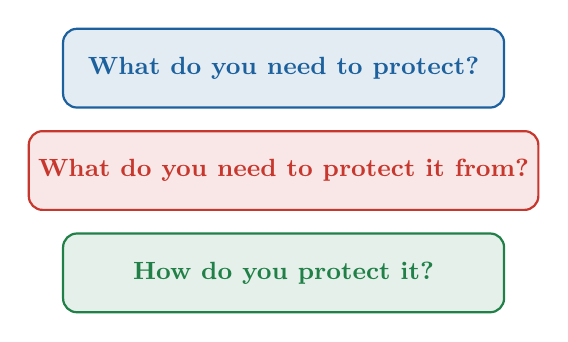
\begin{tikzpicture}
        \foreach \q/\c [count=\i from 0] in {What do you need to protect?/ocean,What do you need to protect it from?/brick,How do you protect it?/leaf!80!black}{
          \node[fill=\c!12,draw=\c,thick,rounded corners=5pt,minimum width=56mm,minimum height=10mm,font=\small\bfseries,text=\c] at (0,-\i*1.3) {\q};
        }
      \end{tikzpicture}
    \end{column}
    \begin{column}{0.54\textwidth}
      \begin{block}{Risk analysis}
        \small The process of \textbf{examining all of your risks} and \textbf{ranking them by severity}.
      \end{block}
      \vspace{2mm}
      \centering
      \textbf{Three major steps}\\[2mm]
      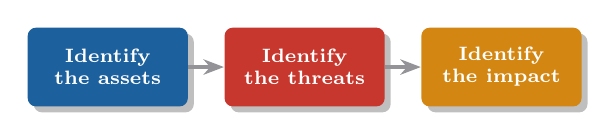
\begin{tikzpicture}
        \foreach \t/\c [count=\i from 0] in {Identify the assets/ocean,Identify the threats/brick,Identify the impact/amber!90!black}{
          \node[fill=\c,text=white,font=\scriptsize\bfseries,rounded corners=3pt,minimum width=20mm,text width=18mm,minimum height=10mm,align=center,drop shadow] (s\i) at (\i*2.5,0) {\t};
        }
        \draw[flow=ink!50] (s0) -- (s1); \draw[flow=ink!50] (s1) -- (s2);
      \end{tikzpicture}
    \end{column}
  \end{columns}
\end{frame}

% ------------------------------------------------------------
\begin{frame}{Step 1: Identifying the Assets}
  \centering
  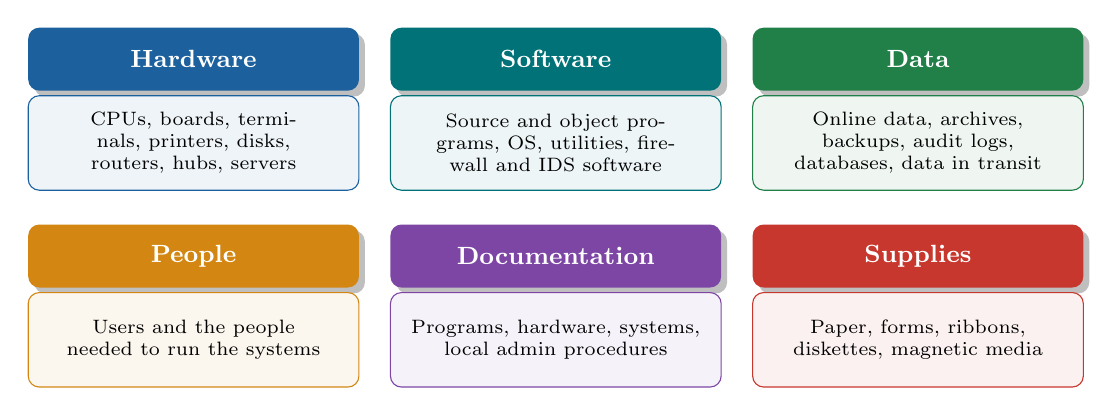
\begin{tikzpicture}
    \foreach \t/\d/\c [count=\i from 0] in {
      Hardware/CPUs\comma{} boards\comma{} terminals\comma{} printers\comma{} disks\comma{} routers\comma{} hubs\comma{} servers/ocean,
      Software/Source and object programs\comma{} OS\comma{} utilities\comma{} firewall and IDS software/aqua!80!black,
      Data/Online data\comma{} archives\comma{} backups\comma{} audit logs\comma{} databases\comma{} data in transit/leaf!80!black,
      People/Users and the people needed to run the systems/amber!90!black,
      Documentation/Programs\comma{} hardware\comma{} systems\comma{} local admin procedures/grape,
      Supplies/Paper\comma{} forms\comma{} ribbons\comma{} diskettes\comma{} magnetic media/brick}
    {
      \pgfmathsetmacro{\x}{mod(\i,3)*4.6}
      \pgfmathsetmacro{\y}{-floor(\i/3)*2.5}
      \node[fill=\c,text=white,font=\small\bfseries,rounded corners=4pt,minimum width=42mm,minimum height=8mm,drop shadow] (h\i) at (\x,\y) {\t};
      \node[draw=\c,fill=\c!7,rounded corners=4pt,minimum width=42mm,minimum height=12mm,text width=39mm,align=center,font=\scriptsize,anchor=north] at ([yshift=-0.5mm]h\i.south) {\d};
    }
  \end{tikzpicture}
  \vspace{2mm}

  {\small List \textbf{all the things that are subject to security threats}.}
\end{frame}

% ------------------------------------------------------------
\begin{frame}{The Asset Inventory}
  \begin{columns}[c]
    \begin{column}{0.5\textwidth}
      \centering
      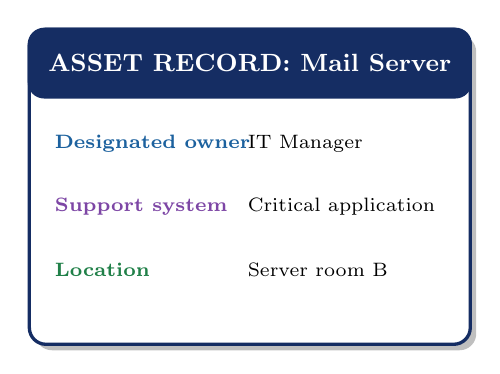
\begin{tikzpicture}
        \node[draw=navy,very thick,fill=white,rounded corners=6pt,minimum width=56mm,minimum height=40mm,drop shadow] (card) at (0,0) {};
        \fill[navy,rounded corners=6pt] ([yshift=-9mm]card.north west) -- (card.north west) -- (card.north east) -- ([yshift=-9mm]card.north east) -- cycle;
        \node[white,font=\small\bfseries] at ([yshift=-4.5mm]card.north) {ASSET RECORD: Mail Server};
        \foreach \k/\v/\c [count=\i from 0] in {Designated owner/IT Manager/ocean,Support system/Critical application/grape,Location/Server room B/leaf!80!black}{
          \node[anchor=west,font=\scriptsize\bfseries,text=\c] at (-2.6,0.55-\i*0.8) {\k};
          \node[anchor=west,font=\scriptsize] at (-0.15,0.55-\i*0.8) {\v};
        }
      \end{tikzpicture}
    \end{column}
    \begin{column}{0.48\textwidth}
      From the asset list, build an \textbf{inventory} with these components for \textbf{each asset}:
      \vspace{2mm}
      \begin{enumerate}\small\setlength{\itemsep}{4pt}
        \item A \textbf{designated owner}
        \item A \textbf{general support system} or \textbf{critical\slash major application}
        \item Its \textbf{physical\slash logical location}
      \end{enumerate}
      \vspace{2mm}
      \begin{block}{Why?}
        \small You cannot protect what you do not know you have, and every asset needs \textbf{someone responsible} for it.
      \end{block}
    \end{column}
  \end{columns}
\end{frame}

% ------------------------------------------------------------
\begin{frame}{Step 2: Identifying the Threats}
  \centering
  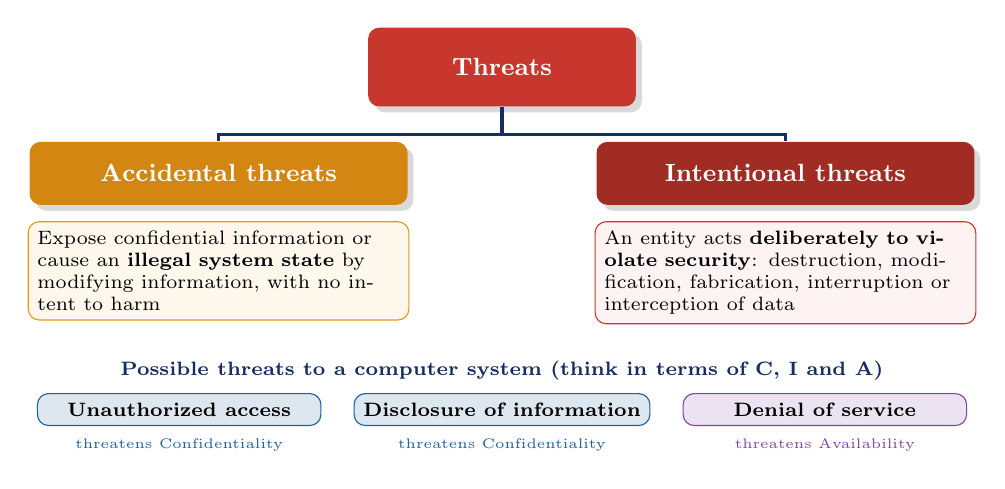
\begin{tikzpicture}
    \node[solid box=brick,minimum width=34mm,minimum height=10mm] (t) at (0,0) {Threats};
    \node[solid box=amber!90!black,minimum width=48mm] (a) at (-3.6,-1.35) {Accidental threats};
    \node[solid box=brick!80!black,minimum width=48mm] (i) at (3.6,-1.35) {Intentional threats};
    \draw[navy,very thick] (t.south) -- ++(0,-0.35) -| (a.north);
    \draw[navy,very thick] (t.south) -- ++(0,-0.35) -| (i.north);
    \node[draw=amber,fill=amber!8,rounded corners,text width=46mm,font=\scriptsize,anchor=north] at ([yshift=-2mm]a.south)
      {Expose confidential information or cause an \textbf{illegal system state} by modifying information, with no intent to harm};
    \node[draw=brick,fill=brick!6,rounded corners,text width=46mm,font=\scriptsize,anchor=north] at ([yshift=-2mm]i.south)
      {An entity acts \textbf{deliberately to violate security}: destruction, modification, fabrication, interruption or interception of data};
    \foreach \t/\g/\c [count=\k from 0] in {Unauthorized access/Confidentiality/ocean,Disclosure of information/Confidentiality/ocean,Denial of service/Availability/grape}{
      \node[fill=\c!15,draw=\c,rounded corners,font=\scriptsize\bfseries,minimum width=36mm] at (\k*4.1-4.1,-4.35) {\t};
      \node[font=\tiny,text=\c] at (\k*4.1-4.1,-4.8) {threatens \g};
    }
    \node[font=\scriptsize\bfseries,text=navy] at (0,-3.85) {Possible threats to a computer system (think in terms of C, I and A)};
  \end{tikzpicture}
\end{frame}

% ------------------------------------------------------------
\begin{frame}{Step 3: Identifying the Impact}
  \centering
  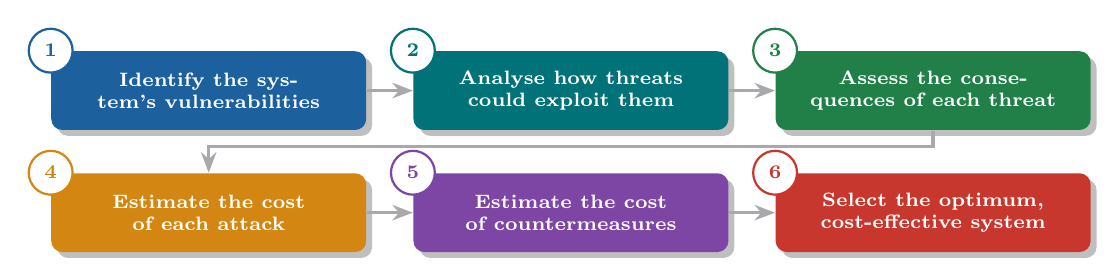
\begin{tikzpicture}
    \foreach \t/\c [count=\i from 0] in {Identify the system's vulnerabilities/ocean,Analyse how threats could exploit them/aqua!80!black,Assess the consequences of each threat/leaf!80!black,Estimate the cost of each attack/amber!90!black,Estimate the cost of countermeasures/grape,Select the optimum\comma{} cost-effective system/brick}{
      \pgfmathsetmacro{\x}{mod(\i,3)*4.6}
      \pgfmathsetmacro{\y}{-floor(\i/3)*1.55}
      \node[fill=\c,text=white,font=\scriptsize\bfseries,rounded corners=4pt,minimum width=40mm,minimum height=10mm,text width=37mm,align=center,drop shadow] (s\i) at (\x,\y) {\t};
      \node[circle,fill=white,draw=\c,thick,font=\scriptsize\bfseries,text=\c,minimum size=5.5mm] at (s\i.north west) {\the\numexpr\i+1\relax};
    }
    \draw[flow=ink!40] (s0) -- (s1); \draw[flow=ink!40] (s1) -- (s2);
    \draw[flow=ink!40] (s2.south) -- ++(0,-0.2) -| (s3.north);
    \draw[flow=ink!40] (s3) -- (s4); \draw[flow=ink!40] (s4) -- (s5);
  \end{tikzpicture}
  \vspace{4mm}
  \begin{alertblock}{A threat that materializes can cause one or more impacts}
    \small \textbullet~Infringement of \textbf{privacy} \qquad \textbullet~\textbf{Financial} loss \qquad \textbullet~\textbf{Disruption} of activities
  \end{alertblock}
\end{frame}

% ------------------------------------------------------------
\begin{frame}{What Is a Threat?}
  \begin{columns}[c]
    \begin{column}{0.5\textwidth}
      \centering
      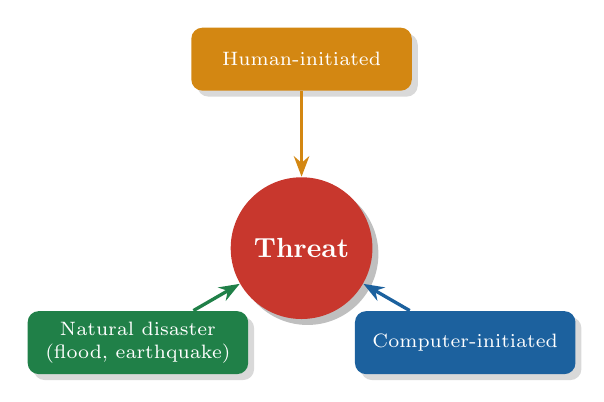
\begin{tikzpicture}
        \node[circle,fill=brick,text=white,font=\bfseries,minimum size=18mm,drop shadow] (t) at (0,0) {Threat};
        \foreach \a/\t/\c in {90/Human-initiated/amber!90!black,-30/Computer-initiated/ocean,210/Natural disaster\\(flood\comma{} earthquake)/leaf!80!black}{
          \node[solid box=\c,minimum width=28mm,font=\scriptsize] (s\a) at (\a:2.4) {\t};
          \draw[\c,very thick,->] (s\a) -- (t);
        }
      \end{tikzpicture}
    \end{column}
    \begin{column}{0.48\textwidth}
      \begin{block}{Definition}
        \small A set of circumstances that has the \textbf{capability of causing loss or harm} to the computer system.
      \end{block}
      \begin{itemize}\small\setlength{\itemsep}{3pt}
        \item Multiprogramming increased what needs protection: system software, memory, shared I/O devices (disks, printers, tape drives), shared programs, networks and data
        \item A threat can be \textbf{accidental} or \textbf{deliberate}
      \end{itemize}
    \end{column}
  \end{columns}
\end{frame}

% ------------------------------------------------------------
\begin{frame}{Four Kinds of Security Breach}
  \centering
  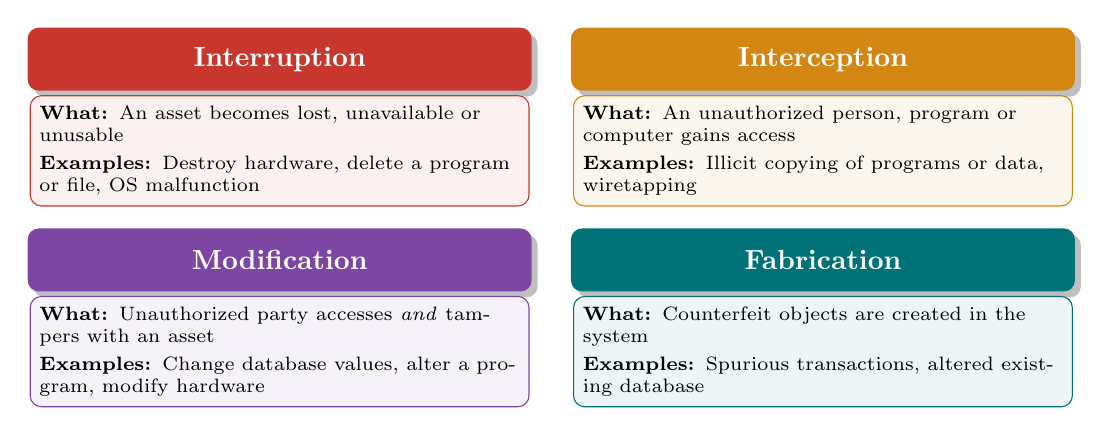
\begin{tikzpicture}
    \foreach \x/\y/\c/\t/\d/\e in {
      0/0/brick/Interruption/An asset becomes lost\comma{} unavailable or unusable/Destroy hardware\comma{} delete a program or file\comma{} OS malfunction,
      6.9/0/amber!90!black/Interception/An unauthorized person\comma{} program or computer gains access/Illicit copying of programs or data\comma{} wiretapping,
      0/-2.55/grape/Modification/Unauthorized party accesses \emph{and} tampers with an asset/Change database values\comma{} alter a program\comma{} modify hardware,
      6.9/-2.55/aqua!80!black/Fabrication/Counterfeit objects are created in the system/Spurious transactions\comma{} altered existing database}
    {
      \node[fill=\c,text=white,rounded corners=4pt,font=\bfseries,minimum width=64mm,minimum height=8mm,drop shadow] (h) at (\x,\y) {\t};
      \node[draw=\c,fill=\c!7,rounded corners=4pt,text width=61mm,minimum height=14mm,font=\scriptsize,anchor=north,align=left] at ([yshift=-0.5mm]h.south)
        {\textbf{What:} \d\\[2pt]\textbf{Examples:} \e};
    }
  \end{tikzpicture}
\end{frame}

% ------------------------------------------------------------
\begin{frame}{What Does an Attacker Need? M--O--M}
  \begin{columns}[c]
    \begin{column}{0.5\textwidth}
      \centering
      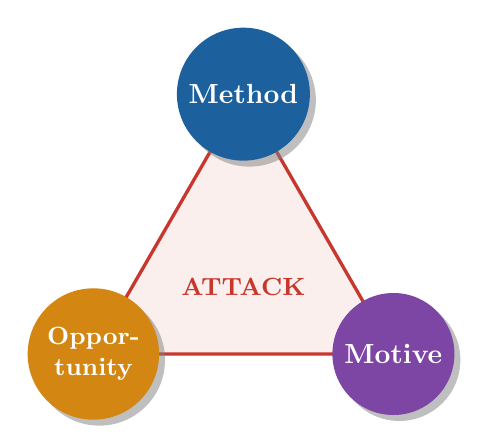
\begin{tikzpicture}
        \coordinate (T) at (90:2.2); \coordinate (L) at (210:2.2); \coordinate (R) at (330:2.2);
        \fill[brick!8,draw=brick,very thick,rounded corners=6pt] (T) -- (L) -- (R) -- cycle;
        \node[circle,fill=ocean,text=white,font=\bfseries,minimum size=15mm,drop shadow] at (T) {Method};
        \node[circle,fill=amber!90!black,text=white,font=\small\bfseries,minimum size=15mm,align=center,drop shadow] at (L) {Oppor-\\tunity};
        \node[circle,fill=grape,text=white,font=\bfseries,minimum size=15mm,drop shadow] at (R) {Motive};
        \node[font=\small\bfseries,text=brick,align=center] at (0,-0.25) {ATTACK};
      \end{tikzpicture}
    \end{column}
    \begin{column}{0.48\textwidth}
      \begin{itemize}\setlength{\itemsep}{8pt}\small
        \item[\textcolor{ocean}{\Large\textbullet}] \textbf{Method}: the tools, skills and knowledge
        \item[\textcolor{amber!90!black}{\Large\textbullet}] \textbf{Opportunity}: the right time and the right access
        \item[\textcolor{grape}{\Large\textbullet}] \textbf{Motive}: the reason to carry out the attack
      \end{itemize}
      \vspace{2mm}
      \begin{exampleblock}{Defender's view}
        \small Take away \textbf{any one} of the three and the attack cannot happen. Limiting \emph{opportunity} is usually the easiest.
      \end{exampleblock}
    \end{column}
  \end{columns}
\end{frame}

% ------------------------------------------------------------
\begin{frame}{Threat, Vulnerability and Control}
  \centering
  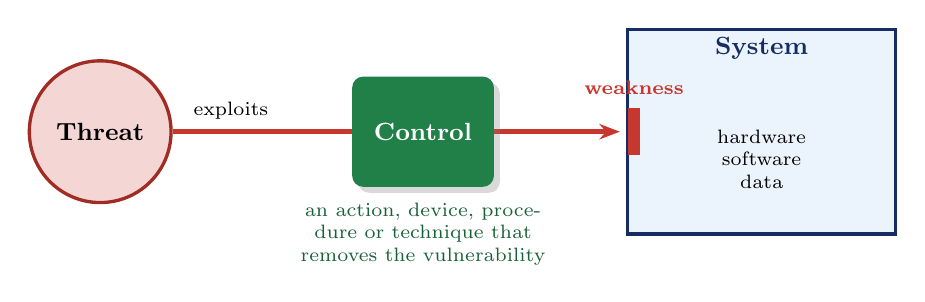
\begin{tikzpicture}
    \node[station=brick,minimum size=18mm] (t) at (0,0) {Threat};
    \node[draw=navy,very thick,fill=sky,minimum width=34mm,minimum height=26mm] (sys) at (8.4,0) {};
    \node[font=\small\bfseries,text=navy,anchor=north] at (sys.north) {System};
    \node[font=\scriptsize,align=center] at (8.4,-0.35) {hardware\\software\\data};
    \fill[brick] (6.7,-0.3) rectangle (6.85,0.3);
    \node[font=\scriptsize\bfseries,text=brick,anchor=south] at (6.78,0.35) {weakness};
    \draw[flow=brick,line width=2pt] (t) -- node[above,font=\scriptsize,pos=0.13]{exploits} (6.6,0);
    \node[solid box=leaf!80!black,minimum width=18mm,minimum height=14mm] (c) at (4.1,0) {Control};
    \node[font=\scriptsize,text=leaf!60!black,text width=40mm,align=center] at (4.1,-1.3) {an action, device, procedure or technique that removes the vulnerability};
  \end{tikzpicture}
  \vspace{3mm}
  \begin{columns}[T]
    \begin{column}{0.48\textwidth}
      \begin{alertblock}{Vulnerability}
        \small A \textbf{weakness} in the system that threats can exploit. It does no harm \textbf{until exploited}. It can lie in \textbf{procedures, design or implementation}.
      \end{alertblock}
    \end{column}
    \begin{column}{0.48\textwidth}
      \begin{exampleblock}{Control}
        \small A \textbf{protective measure} that limits or \textbf{eliminates} a vulnerability, and so \textbf{blocks} the threat.
      \end{exampleblock}
    \end{column}
  \end{columns}
\end{frame}

% ------------------------------------------------------------
\begin{frame}{Everyday Vulnerabilities}
  \centering
  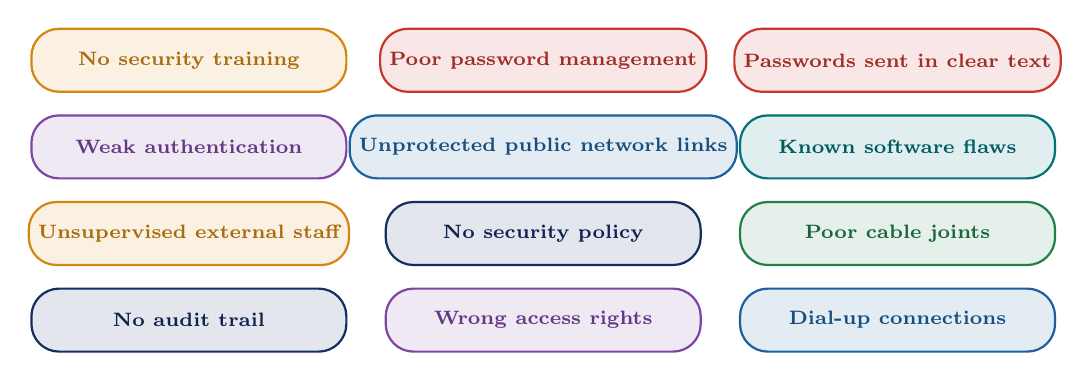
\begin{tikzpicture}
    \foreach \t/\x/\y/\c in {
      No security training/0/0/amber!90!black,
      Poor password management/4.5/0/brick,
      Passwords sent in clear text/9/0/brick,
      Weak authentication/0/-1.1/grape,
      Unprotected public network links/4.5/-1.1/ocean,
      Known software flaws/9/-1.1/aqua!80!black,
      Unsupervised external staff/0/-2.2/amber!90!black,
      No security policy/4.5/-2.2/navy,
      Poor cable joints/9/-2.2/leaf!80!black,
      No audit trail/0/-3.3/navy,
      Wrong access rights/4.5/-3.3/grape,
      Dial-up connections/9/-3.3/ocean}
    {
      \node[fill=\c!12,draw=\c,thick,rounded corners=10pt,minimum width=40mm,minimum height=8mm,font=\scriptsize\bfseries,text=\c!80!black] at (\x,\y) {\t};
    }
  \end{tikzpicture}
  \vspace{3mm}

  {\small Also: inadequate recruitment procedures, insufficient preventive maintenance, inadequate system management.}
\end{frame}

% ------------------------------------------------------------
\begin{frame}{Vulnerabilities by Component}
  \centering
  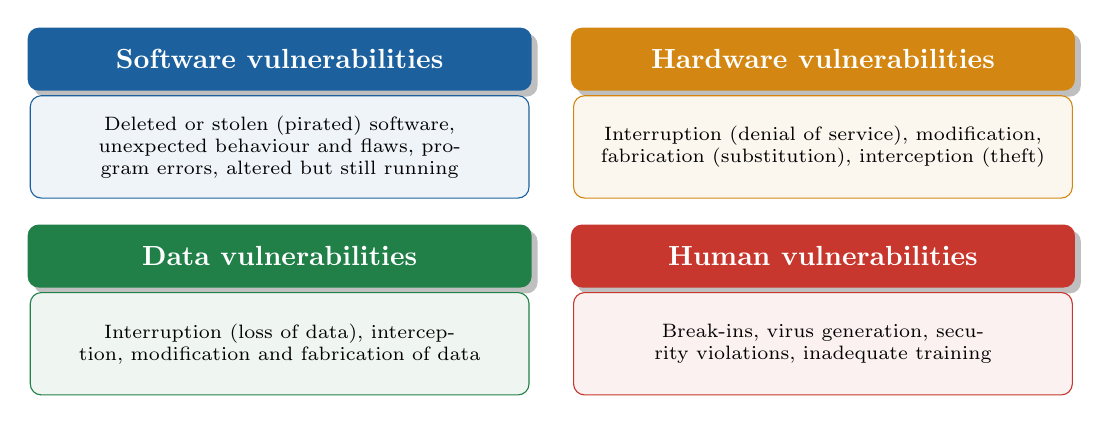
\begin{tikzpicture}
    \foreach \x/\y/\c/\t/\d in {
      0/0/ocean/Software/Deleted or stolen (pirated) software\comma{} unexpected behaviour and flaws\comma{} program errors\comma{} altered but still running,
      6.9/0/amber!90!black/Hardware/Interruption (denial of service)\comma{} modification\comma{} fabrication (substitution)\comma{} interception (theft),
      0/-2.5/leaf!80!black/Data/Interruption (loss of data)\comma{} interception\comma{} modification and fabrication of data,
      6.9/-2.5/brick/Human/Break-ins\comma{} virus generation\comma{} security violations\comma{} inadequate training}
    {
      \node[fill=\c,text=white,rounded corners=4pt,font=\bfseries,minimum width=64mm,minimum height=8mm,drop shadow] (h) at (\x,\y) {\t\ vulnerabilities};
      \node[draw=\c,fill=\c!7,rounded corners=4pt,text width=61mm,minimum height=13mm,font=\scriptsize,anchor=north,align=center] at ([yshift=-0.5mm]h.south) {\d};
    }
  \end{tikzpicture}
\end{frame}

% ------------------------------------------------------------
\begin{frame}{User Authentication: Three Qualities}
  \centering
  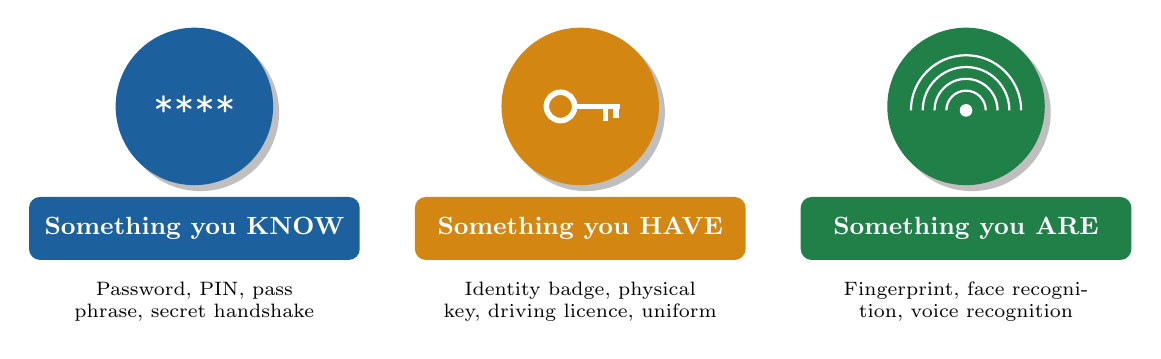
\begin{tikzpicture}
    \foreach \x/\c/\t/\q/\e [count=\i] in {
      0/ocean/Something you KNOW/know/Password\comma{} PIN\comma{} pass phrase\comma{} secret handshake,
      4.9/amber!90!black/Something you HAVE/have/Identity badge\comma{} physical key\comma{} driving licence\comma{} uniform,
      9.8/leaf!80!black/Something you ARE/are/Fingerprint\comma{} face recognition\comma{} voice recognition}
    {
      \node[circle,fill=\c,minimum size=20mm,drop shadow] (c\i) at (\x,0) {};
      \node[fill=\c,text=white,rounded corners=4pt,font=\small\bfseries,minimum width=42mm,minimum height=8mm] (h\i) at (\x,-1.55) {\t};
      \node[font=\scriptsize,text width=40mm,align=center,below=1.5mm of h\i] {\e};
    }
    % icons
    \node[white,font=\Large\ttfamily\bfseries] at (0,0) {****};
    \pic[scale=1.5] at (4.65,0) {key=white};
    \foreach \r in {0.25,0.4,0.55,0.7} \draw[white,thick] (9.8,-0.05) ++(-\r,0) arc (180:0:\r);
    \fill[white] (9.8,-0.05) circle (0.08);
  \end{tikzpicture}
  \vspace{3mm}
  \begin{exampleblock}{Combine for stronger authentication}
    \small Two or more methods together give \textbf{more solid} authentication, e.g.\ an \textbf{identity card + PIN} (have + know), as at an ATM.
  \end{exampleblock}
\end{frame}

% ------------------------------------------------------------
\begin{frame}{Who Has Access to What? MAC vs.\ DAC}
  \begin{columns}[T]
    \begin{column}{0.49\textwidth}
      \centering\textbf{\textcolor{navy}{Mandatory Access Control (MAC)}}\\[2mm]
      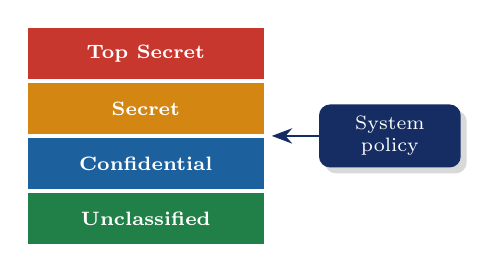
\begin{tikzpicture}
        \foreach \t/\c [count=\i from 0] in {Top Secret/brick,Secret/amber!90!black,Confidential/ocean,Unclassified/leaf!80!black}
          \node[fill=\c,text=white,font=\scriptsize\bfseries,minimum width=30mm-\i*0mm,minimum height=6.5mm] at (0,-\i*0.7) {\t};
        \node[solid box=navy,minimum width=18mm,font=\scriptsize] at (3.1,-1.05) {System\\policy};
        \draw[->,thick,navy] (2.2,-1.05) -- (1.6,-1.05);
      \end{tikzpicture}\\[1mm]
      {\small A policy for systems with \textbf{highly secret or sensitive} information. Access follows fixed labels set by the \textbf{system}. Typically used by \textbf{government agencies}.}
    \end{column}
    \begin{column}{0.49\textwidth}
      \centering\textbf{\textcolor{grape}{Discretionary Access Control (DAC)}}\\[2mm]
      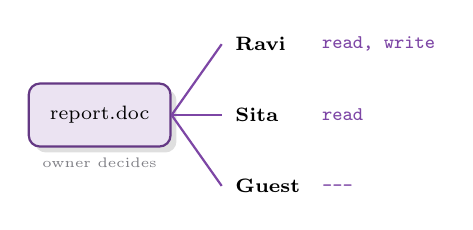
\begin{tikzpicture}
        \node[box=grape,minimum width=18mm,font=\scriptsize] (f) at (0,0) {report.doc};
        \foreach \u/\r/\y in {Ravi/read\comma{} write/0.9,Sita/read/0,Guest/---/-0.9}{
          \node[anchor=west,font=\scriptsize\bfseries] at (1.6,\y) {\u};
          \node[anchor=west,font=\scriptsize\ttfamily,text=grape] at (2.7,\y) {\r};
          \draw[grape,thick] (f.east) -- (1.55,\y);
        }
        \node[font=\tiny,text=ink!60] at (0,-0.6) {owner decides};
      \end{tikzpicture}\\[1mm]
      {\small Uses the \textbf{identity of the user or group}. \emph{Discretionary}: the administrator decides \textbf{who} has access and \textbf{what type}: create, write, read, update or delete.}
    \end{column}
  \end{columns}
\end{frame}

% ------------------------------------------------------------
\begin{frame}{Authentication and Biometrics}
  \centering
  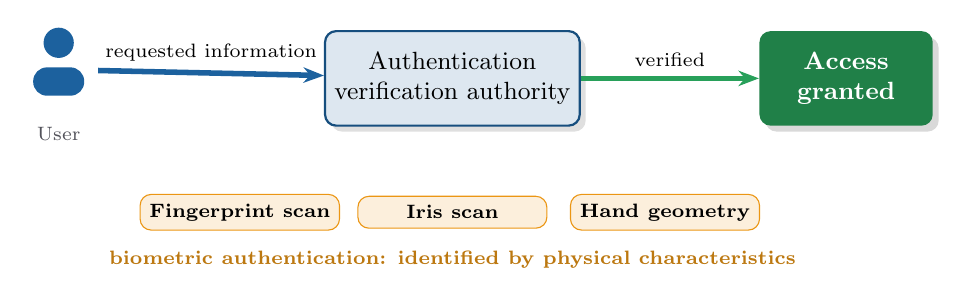
\begin{tikzpicture}
    \pic[scale=1.2] at (0,0) {person=ocean}; \node[tag] at (0,-0.6) {User};
    \node[box=ocean,minimum width=26mm,minimum height=12mm] (v) at (5,0.1) {Authentication\\verification authority};
    \node[solid box=leaf!80!black,minimum width=22mm,minimum height=12mm] (ok) at (10,0.1) {Access\\granted};
    \draw[flow=ocean,line width=2pt] (0.5,0.2) -- node[above,font=\scriptsize]{requested information} (v);
    \draw[flow=leaf,line width=2pt] (v) -- node[above,font=\scriptsize]{verified} (ok);
    \foreach \t/\x in {Fingerprint scan/2.3,Iris scan/5,Hand geometry/7.7}{
      \node[fill=amber!15,draw=amber,rounded corners,font=\scriptsize\bfseries,minimum width=24mm] at (\x,-1.6) {\t};
    }
    \node[font=\scriptsize\bfseries,text=amber!80!black] at (5,-2.2) {biometric authentication: identified by physical characteristics};
  \end{tikzpicture}
  \vspace{3mm}
  \begin{itemize}\small
    \item Authentication occurs when a user \textbf{provides the requested information} to a verification authority
    \item The \textbf{traditional} method is a \textbf{password}
    \item For more \textbf{reliability}, use biometrics: the user is identified by who they physically \emph{are}, not just digitally
  \end{itemize}
\end{frame}

% ------------------------------------------------------------
\begin{frame}{Hardware Token: Challenge and Response}
  \centering
  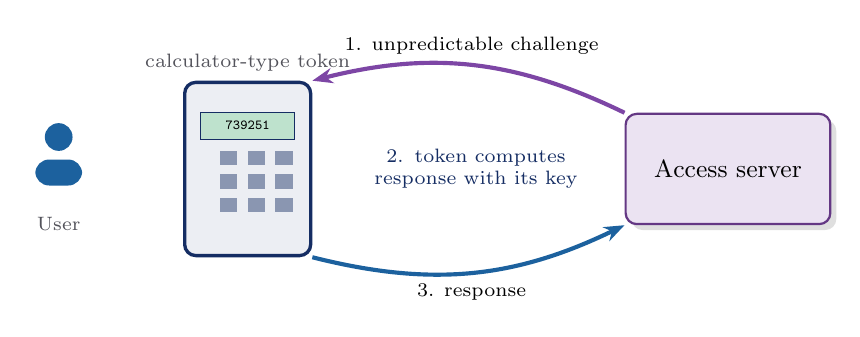
\begin{tikzpicture}
    \pic[scale=1.1] at (0,0) {person=ocean}; \node[tag] at (0,-0.6) {User};
    % token
    \node[draw=navy,very thick,fill=navy!8,rounded corners=4pt,minimum width=16mm,minimum height=22mm] (tok) at (2.4,0.1) {};
    \node[fill=leaf!30,draw=navy,font=\tiny\ttfamily,minimum width=12mm] at (2.4,0.65) {739251};
    \foreach \r in {0,1,2} \foreach \c in {0,1,2} \fill[navy!50] (2.05+\c*0.35,0.15-\r*0.3) rectangle ++(0.22,0.18);
    \node[tag] at (2.4,1.45) {calculator-type token};
    \node[box=grape,minimum width=26mm,minimum height=14mm] (srv) at (8.5,0.1) {Access server};
    \draw[flow=grape,line width=1.5pt] (srv.north west) to[bend right=20] node[above,font=\scriptsize]{1. unpredictable challenge} (tok.north east);
    \draw[flow=ocean,line width=1.5pt] (tok.south east) to[bend right=20] node[below,font=\scriptsize]{3. response} (srv.south west);
    \node[font=\scriptsize,text=navy,text width=28mm,align=center] at (5.3,0.1) {2. token computes response with its key};
  \end{tikzpicture}
  \vspace{3mm}
  \begin{columns}[T]
    \begin{column}{0.5\textwidth}
      \begin{block}{Authentication token}
        \small A \textbf{portable device} used for authenticating a user.
      \end{block}
    \end{column}
    \begin{column}{0.46\textwidth}
      \begin{itemize}\small
        \item Token and server hold \textbf{identical security keys or algorithms}
        \item The user types the challenge into the token and sends back the response
      \end{itemize}
    \end{column}
  \end{columns}
\end{frame}

% ------------------------------------------------------------
\begin{frame}{Hardware Token: Time-Based}
  \centering
  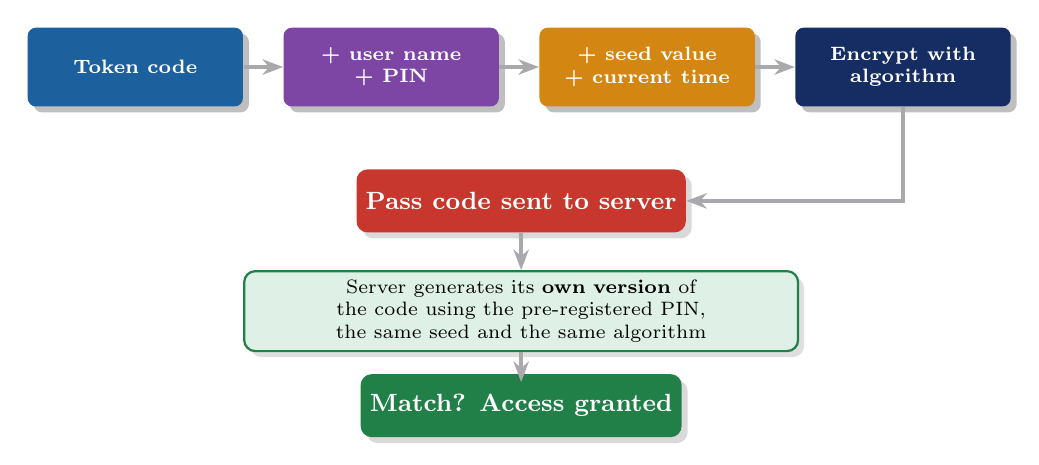
\begin{tikzpicture}
    \foreach \t/\c [count=\i from 0] in {Token code/ocean,+ user name + PIN/grape,+ seed value + current time/amber!90!black,Encrypt with algorithm/navy}{
      \node[fill=\c,text=white,font=\scriptsize\bfseries,rounded corners=3pt,minimum width=27mm,text width=25mm,minimum height=10mm,align=center,drop shadow] (s\i) at (\i*3.25,1.2) {\t};
    }
    \foreach \i [evaluate=\i as \j using int(\i+1)] in {0,1,2} \draw[flow=ink!40] (s\i) -- (s\j);
    \node[solid box=brick,minimum width=26mm] (pc) at (4.9,-0.5) {Pass code sent to server};
    \draw[flow=ink!40] (s3.south) |- (pc.east);
    \node[box=leaf,minimum width=70mm,font=\scriptsize,text width=68mm,align=center] (sv) at (4.9,-1.9) {Server generates its \textbf{own version} of the code using the pre-registered PIN, the same seed and the same algorithm};
    \draw[flow=ink!40] (pc) -- (sv);
    \node[solid box=leaf!80!black,minimum width=26mm] at (4.9,-3.1) {Match? Access granted};
    \draw[flow=ink!40] (sv) -- (4.9,-2.8);
  \end{tikzpicture}
  \vspace{1mm}

  {\small The token and the server use an \textbf{identical algorithm}. Because the current time is part of the input, each pass code is \textbf{valid only briefly}.}
\end{frame}

% ------------------------------------------------------------
\begin{frame}{Software Tokens}
  \begin{columns}[c]
    \begin{column}{0.48\textwidth}
      \centering
      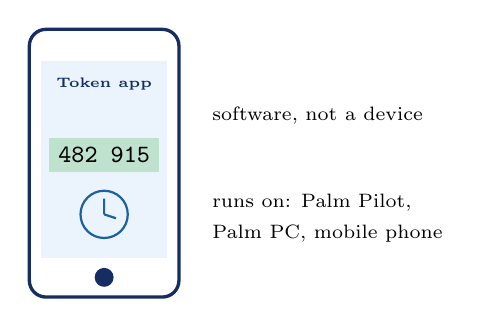
\begin{tikzpicture}
        \draw[navy,very thick,fill=white,rounded corners=6pt] (0,0) rectangle (1.9,3.4);
        \fill[sky] (0.15,0.5) rectangle (1.75,3.0);
        \fill[navy] (0.95,0.25) circle (0.12);
        \node[font=\tiny\bfseries,text=navy] at (0.95,2.7) {Token app};
        \node[fill=leaf!30,font=\small\ttfamily\bfseries] at (0.95,1.8) {482 915};
        \draw[ocean,thick] (0.95,1.05) circle (0.3);
        \draw[ocean,thick] (0.95,1.05) -- (0.95,1.25) (0.95,1.05) -- (1.1,1.0);
        \node[font=\scriptsize,right] at (2.2,2.3) {software, not a device};
        \node[font=\scriptsize,right] at (2.2,1.2) {runs on: Palm Pilot,};
        \node[font=\scriptsize,right] at (2.2,0.8) {Palm PC, mobile phone};
      \end{tikzpicture}
    \end{column}
    \begin{column}{0.5\textwidth}
      \begin{block}{Software token}
        \small An authentication process using \textbf{portable devices} (Palm Pilot, Palm PC, wireless telephone) that carry the \textbf{embedded software}.
      \end{block}
      \vspace{2mm}
      \begin{itemize}\small\setlength{\itemsep}{3pt}
        \item Chosen when an organization does \textbf{not wish to buy hardware tokens}
        \item Today's authenticator apps on smartphones are modern software tokens
      \end{itemize}
    \end{column}
  \end{columns}
\end{frame}

% ============================================================
\setcounter{section}{6}
\section{Multi Level Model of Security}
% ============================================================

\begin{frame}{Security System and Facilities}
  \begin{columns}[c]
    \begin{column}{0.52\textwidth}
      \centering
      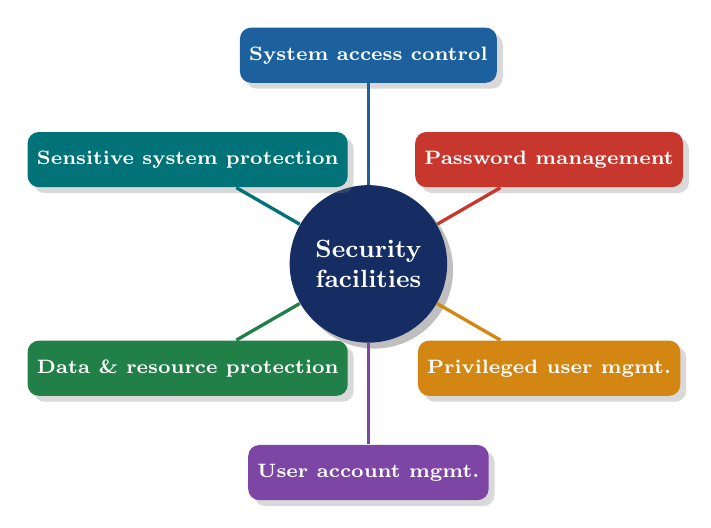
\begin{tikzpicture}
        \node[circle,fill=navy,text=white,font=\small\bfseries,minimum size=20mm,align=center,drop shadow] (c) at (0,0) {Security\\facilities};
        \foreach \a/\t/\c in {90/System access control/ocean,30/Password management/brick,-30/Privileged user mgmt./amber!90!black,-90/User account mgmt./grape,-150/Data \& resource protection/leaf!80!black,150/Sensitive system protection/aqua!80!black}{
          \node[solid box=\c,minimum width=30mm,minimum height=7mm,font=\scriptsize\bfseries] (s\a) at (\a:2.65) {\t};
          \draw[\c,very thick] (c) -- (s\a);
        }
      \end{tikzpicture}
    \end{column}
    \begin{column}{0.46\textwidth}
      \begin{itemize}\small\setlength{\itemsep}{5pt}
        \item Security controls should be installed and maintained on \textbf{each computer system or node}
        \item Goal: stop \textbf{unauthorized users} entering the system and stop \textbf{unauthorized access} to data
        \item Software and resources are reachable \textbf{only after authentication}
      \end{itemize}
    \end{column}
  \end{columns}
\end{frame}

% ------------------------------------------------------------
\begin{frame}{System Access Control}
  \begin{columns}[T]
    \begin{column}{0.49\textwidth}
      \begin{block}{Who can get in}
        \small
        \begin{itemize}\setlength{\itemsep}{2pt}
          \item Access to memory, storage, sensitive utilities and files is on a \textbf{``need-to-use'' basis}
          \item Access-control software must restrict access; \textbf{avoid common passwords} like ``administrative'', ``president'', ``game''
          \item Access guidelines are \textbf{documented and implemented}
          \item Each user gets a \textbf{unique user ID}
        \end{itemize}
      \end{block}
    \end{column}
    \begin{column}{0.49\textwidth}
      \begin{exampleblock}{What the system must do}
        \small
        \begin{itemize}\setlength{\itemsep}{2pt}
          \item \textbf{Encrypt} stored passwords with proven algorithms
          \item \textbf{Auto time-out} for inactive terminals
          \item Log an \textbf{audit trail} of sensitive actions, and protect it from change or deletion
          \item Log and monitor \textbf{remote users}
          \item Automate security start-up and shutdown
          \item Protect sensitive OS files with proven tools
        \end{itemize}
      \end{exampleblock}
    \end{column}
  \end{columns}
\end{frame}

% ------------------------------------------------------------
\begin{frame}{Password Management Rules}
  \centering
  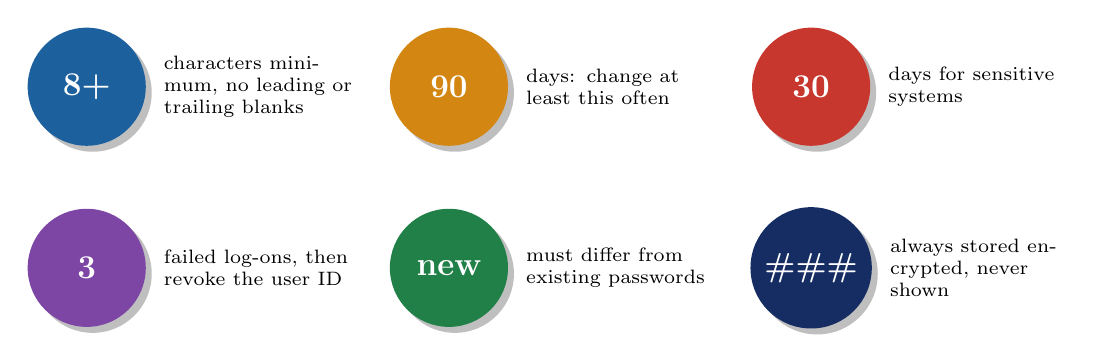
\begin{tikzpicture}
    \foreach \v/\t/\c [count=\i from 0] in {
      8+/characters minimum\comma{} no leading or trailing blanks/ocean,
      90/days: change at least this often/amber!90!black,
      30/days for sensitive systems/brick,
      3/failed log-ons\comma{} then revoke the user ID/grape,
      new/must differ from existing passwords/leaf!80!black,
      \#\#\#/always stored encrypted\comma{} never shown/navy}
    {
      \pgfmathsetmacro{\x}{mod(\i,3)*4.6}
      \pgfmathsetmacro{\y}{-floor(\i/3)*2.3}
      \node[circle,fill=\c,text=white,font=\large\bfseries,minimum size=15mm,drop shadow] (c\i) at (\x-1.4,\y) {\v};
      \node[anchor=west,font=\scriptsize,text width=24mm] at ([xshift=1mm]c\i.east) {\t};
    }
  \end{tikzpicture}
  \vspace{3mm}
  \begin{alertblock}{Also}
    \small Do not share, display or print passwords \,$\cdot$\, avoid easy-to-guess passwords \,$\cdot$\, resist \textbf{dictionary attacks} and known cracking tools
  \end{alertblock}
\end{frame}

% ------------------------------------------------------------
\begin{frame}{Weak vs.\ Strong Passwords}
  \begin{columns}[T]
    \begin{column}{0.49\textwidth}
      \centering\textbf{\textcolor{brick}{Weak: guessed in seconds}}\\[2mm]
      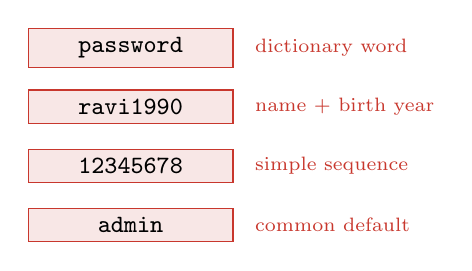
\begin{tikzpicture}
        \foreach \p/\w [count=\i from 0] in {password/dictionary word,ravi1990/name + birth year,12345678/simple sequence,admin/common default}{
          \node[fill=brick!12,draw=brick,font=\small\ttfamily,minimum width=26mm,anchor=east] at (0,-\i*0.75) {\p};
          \node[font=\scriptsize,anchor=west,text=brick] at (0.15,-\i*0.75) {\w};
        }
      \end{tikzpicture}
    \end{column}
    \begin{column}{0.49\textwidth}
      \centering\textbf{\textcolor{leaf!70!black}{Strong: follows the rules}}\\[2mm]
      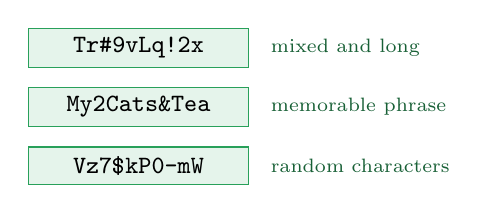
\begin{tikzpicture}
        \foreach \p/\w [count=\i from 0] in {Tr\#9vLq!2x/mixed and long,My2Cats\&Tea/memorable phrase,Vz7\$kP0-mW/random characters}{
          \node[fill=leaf!12,draw=leaf,font=\small\ttfamily,minimum width=28mm,anchor=east] at (0,-\i*0.75) {\p};
          \node[font=\scriptsize,anchor=west,text=leaf!60!black] at (0.15,-\i*0.75) {\w};
        }
      \end{tikzpicture}
    \end{column}
  \end{columns}
  \vspace{4mm}
  \centering
  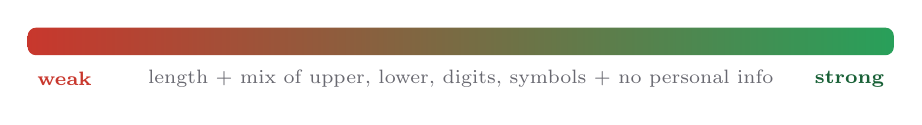
\begin{tikzpicture}
    \shade[left color=brick,right color=leaf,rounded corners=3pt] (0,0) rectangle (11,0.35);
    \node[font=\scriptsize\bfseries,text=brick,anchor=west] at (0,-0.3) {weak};
    \node[font=\scriptsize\bfseries,text=leaf!60!black,anchor=east] at (11,-0.3) {strong};
    \node[font=\scriptsize,text=ink!70] at (5.5,-0.3) {length + mix of upper, lower, digits, symbols + no personal info};
  \end{tikzpicture}
\end{frame}

% ------------------------------------------------------------
\begin{frame}{Privileged Users and User Accounts}
  \begin{columns}[T]
    \begin{column}{0.4\textwidth}
      \begin{block}{Privileged user management}
        \small
        \begin{itemize}\setlength{\itemsep}{2pt}
          \item Privileges only on a \textbf{need-to-use} basis
          \item Log-in available \textbf{only from the console}
          \item Maintain an \textbf{audit log}
        \end{itemize}
      \end{block}
    \end{column}
    \begin{column}{0.58\textwidth}
      \centering\textbf{\textcolor{grape}{User account life cycle}}\\[2mm]
      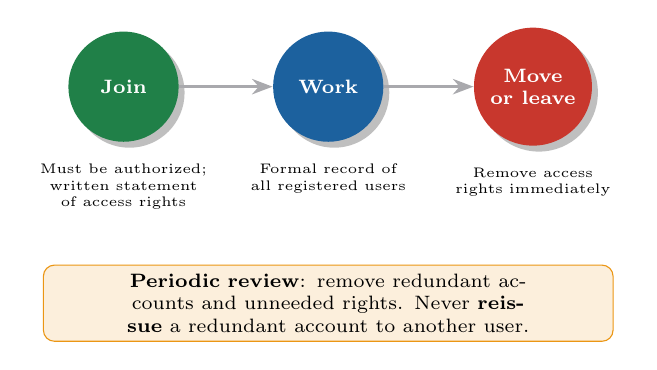
\begin{tikzpicture}
        \foreach \t/\d/\c [count=\i from 0] in {Join/Must be authorized; written statement of access rights/leaf!80!black,Work/Formal record of all registered users/ocean,Move\\or leave/Remove access rights immediately/brick}{
          \node[circle,fill=\c,text=white,font=\scriptsize\bfseries,minimum size=14mm,text width=11mm,align=center,drop shadow] (c\i) at (\i*2.6,0) {\t};
          \node[font=\tiny,text width=22mm,align=center,below=1.5mm of c\i] {\d};
        }
        \draw[flow=ink!40] (c0) -- (c1); \draw[flow=ink!40] (c1) -- (c2);
        \node[fill=amber!15,draw=amber,rounded corners,font=\scriptsize,text width=70mm,align=center] at (2.6,-2.75) {\textbf{Periodic review}: remove redundant accounts and unneeded rights. Never \textbf{reissue} a redundant account to another user.};
      \end{tikzpicture}
    \end{column}
  \end{columns}
\end{frame}

% ------------------------------------------------------------
\begin{frame}{Data, Resource and Sensitive System Protection}
  \begin{columns}[T]
    \begin{column}{0.49\textwidth}
      \begin{block}{Data and resource protection}
        \small
        \begin{itemize}\setlength{\itemsep}{2pt}
          \item Every piece of information gets an \textbf{owner} responsible for its integrity
          \item Assignment of responsibility is \textbf{formal}
          \item \textbf{Top management} supervises the whole allocation process
        \end{itemize}
      \end{block}
      \centering
      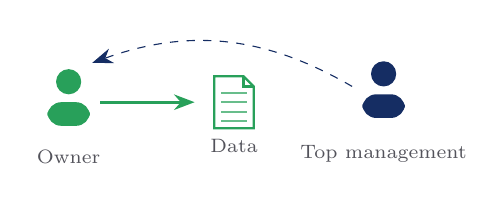
\begin{tikzpicture}
        \pic at (0,0) {person=leaf}; \node[tag] at (0,-0.5) {Owner};
        \draw[flow=leaf] (0.4,0.2) -- (1.6,0.2);
        \pic at (2.1,0.2) {doc=leaf}; \node[tag] at (2.1,-0.35) {Data};
        \pic at (4,0.1) {person=navy}; \node[tag] at (4,-0.45) {Top management};
        \draw[navy,dashed,->] (3.6,0.4) to[bend right=25] (0.3,0.7);
      \end{tikzpicture}
    \end{column}
    \begin{column}{0.49\textwidth}
      \begin{alertblock}{Sensitive system protection}
        \small
        \begin{itemize}\setlength{\itemsep}{2pt}
          \item Security tokens, smart cards and biometrics (iris, fingerprint) \textbf{complement passwords}
          \item \textbf{Encryption} protects the integrity and confidentiality of sensitive data
        \end{itemize}
      \end{alertblock}
      \centering
      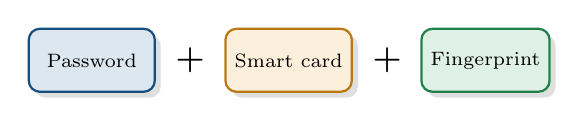
\begin{tikzpicture}
        \node[box=ocean,minimum width=16mm,font=\scriptsize] at (0,0) {Password};
        \node[font=\large\bfseries] at (1.25,0) {+};
        \node[box=amber,minimum width=16mm,font=\scriptsize] at (2.5,0) {Smart card};
        \node[font=\large\bfseries] at (3.75,0) {+};
        \node[box=leaf,minimum width=16mm,font=\scriptsize] at (5,0) {Fingerprint};
      \end{tikzpicture}
    \end{column}
  \end{columns}
\end{frame}

% ------------------------------------------------------------
\begin{frame}{Data Backup and Off-Site Retention}
  \centering
  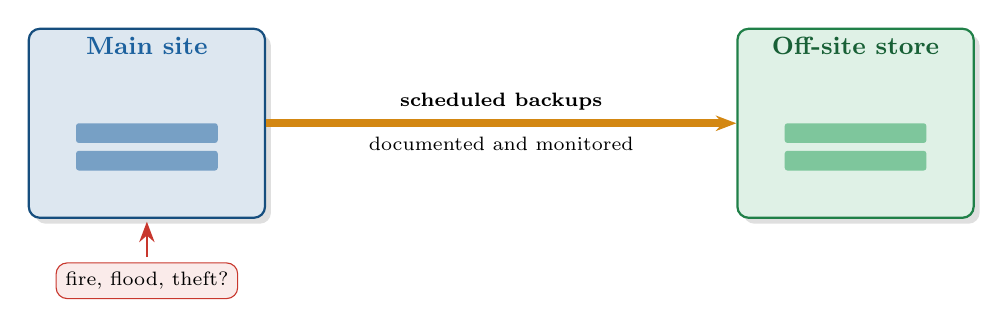
\begin{tikzpicture}
    \node[box=ocean,minimum width=30mm,minimum height=24mm] (main) at (0,0) {};
    \node[font=\small\bfseries,text=ocean,anchor=north] at (main.north) {Main site};
    \foreach \y in {-0.25,-0.6} \fill[ocean!60,rounded corners=1pt] (-0.9,\y) rectangle (0.9,\y+0.25);
    \node[box=leaf,minimum width=30mm,minimum height=24mm] (off) at (9,0) {};
    \node[font=\small\bfseries,text=leaf!60!black,anchor=north] at (off.north) {Off-site store};
    \foreach \y in {-0.25,-0.6} \fill[leaf!60,rounded corners=1pt] (8.1,\y) rectangle (9.9,\y+0.25);
    \draw[flow=amber!90!black,line width=3pt] (main) -- node[above,font=\scriptsize\bfseries]{scheduled backups} node[below,font=\scriptsize]{documented and monitored} (off);
    \node[fill=brick!10,draw=brick,rounded corners,font=\scriptsize,align=center] at (0,-2.0) {fire, flood, theft?};
    \draw[brick,thick,->] (0,-1.7) -- (0,-1.25);
  \end{tikzpicture}
  \vspace{3mm}
  \begin{block}{Keep up-to-date backups of critical items}
    \small Data files \,$\cdot$\, utilities and programs \,$\cdot$\, databases \,$\cdot$\, operating system code \,$\cdot$\, \textbf{encryption keys} \,$\cdot$\, documentation \,$\cdot$\, full and incremental backups on a schedule
  \end{block}
\end{frame}

% ------------------------------------------------------------
\begin{frame}{Firewall: The First Line of Defence}
  \begin{columns}[c]
    \begin{column}{0.54\textwidth}
      \centering
      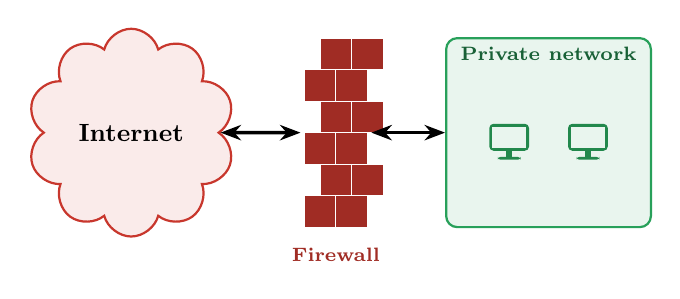
\begin{tikzpicture}
        \node[cloud,cloud puffs=10,draw=brick,fill=brick!10,thick,minimum width=2.5cm,minimum height=1.6cm,font=\small\bfseries] (net) at (0,0) {Internet};
        % brick wall
        \begin{scope}[shift={(2.4,-1.2)}]
          \foreach \r in {0,...,5}{
            \pgfmathsetmacro{\off}{mod(\r,2)*0.2}
            \foreach \c in {0,1}
              \draw[white,fill=brick!80!black] (\off+\c*0.4-0.2,\r*0.4) rectangle ++(0.4,0.4);
          }
        \end{scope}
        \node[font=\scriptsize\bfseries,text=brick!80!black] at (2.6,-1.55) {Firewall};
        \node[draw=leaf,fill=leaf!10,thick,rounded corners,minimum width=26mm,minimum height=24mm] (lan) at (5.3,0) {};
        \node[font=\scriptsize\bfseries,text=leaf!60!black,anchor=north] at (lan.north) {Private network};
        \pic[scale=0.6] at (4.8,-0.2) {pc=leaf}; \pic[scale=0.6] at (5.8,-0.2) {pc=leaf};
        \draw[<->,very thick] (net) -- (2.15,0);
        \draw[<->,very thick] (3.05,0) -- (lan);
      \end{tikzpicture}
    \end{column}
    \begin{column}{0.44\textwidth}
      \begin{itemize}\small\setlength{\itemsep}{4pt}
        \item \textbf{All packets} entering the network must pass through this point
        \item A modern firewall is a \textbf{system of applications and hardware} working together
        \item It combines:
      \end{itemize}
      
\begin{tikzpicture}
        \foreach \t/\c [count=\i from 0] in {Packet filtering/ocean,NAT/grape,Proxy services/amber!90!black}
          \node[solid box=\c,minimum width=18mm,font=\scriptsize] at (\i*2.05,0) {\t};
      \end{tikzpicture}
    \end{column}
  \end{columns}
\end{frame}

% ------------------------------------------------------------
\begin{frame}{Packet Filtering Router}
  \centering
  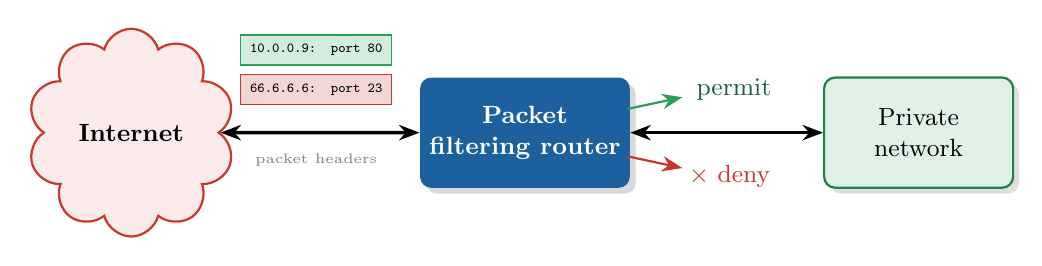
\begin{tikzpicture}
    \node[cloud,cloud puffs=10,draw=brick,fill=brick!10,thick,minimum width=2.5cm,minimum height=1.5cm,font=\small\bfseries] (net) at (0,0) {Internet};
    \node[solid box=ocean,minimum width=26mm,minimum height=14mm] (pf) at (5,0) {Packet\\filtering router};
    \node[box=leaf,minimum width=24mm,minimum height=14mm] (pn) at (10,0) {Private\\network};
    \draw[<->,very thick] (net) -- (pf); \draw[<->,very thick] (pf) -- (pn);
    \node[fill=leaf!20,draw=leaf,font=\tiny\ttfamily] at (2.35,1.05) {10.0.0.9: port 80};
    \node[fill=brick!20,draw=brick,font=\tiny\ttfamily] at (2.35,0.55) {66.6.6.6: port 23};
    \node[font=\tiny,text=ink!60] at (2.35,-0.35) {packet headers};
    \node[font=\small,text=leaf!60!black] at (7.6,0.55) {\checkmark\ permit};
    \node[font=\small,text=brick] at (7.6,-0.55) {$\times$ deny};
    \draw[leaf,thick,->] (6.3,0.3) -- (7.0,0.45);
    \draw[brick,thick,->] (6.3,-0.3) -- (7.0,-0.45);
  \end{tikzpicture}
  \vspace{3mm}
  \begin{columns}[T]
    \begin{column}{0.5\textwidth}
      \begin{block}{How it works}
        \small Looks at the \textbf{header information} of each packet and \textbf{permits or denies} it based on simple rules.
      \end{block}
    \end{column}
    \begin{column}{0.46\textwidth}
      \begin{itemize}\small
        \item The \textbf{first type} of firewall used by many organizations
        \item Usually implemented on a \textbf{router}
        \item Fast, but sees only headers, not content
      \end{itemize}
    \end{column}
  \end{columns}
\end{frame}

% ------------------------------------------------------------
\begin{frame}{Proxy Server (Application Gateway)}
  \centering
  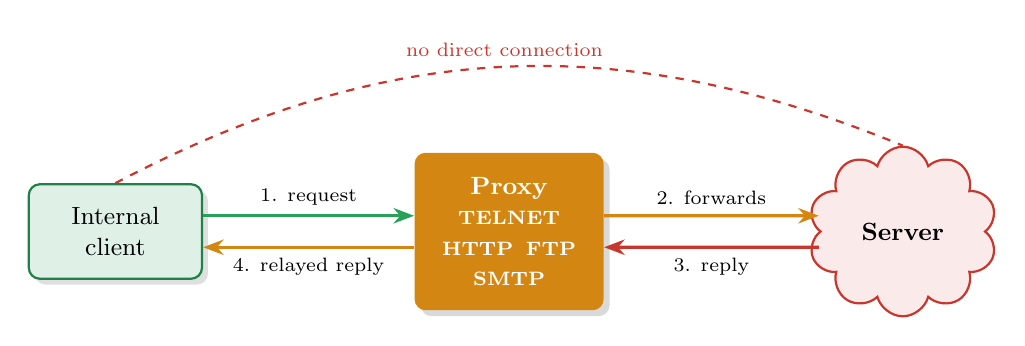
\begin{tikzpicture}
    \node[box=leaf,minimum width=22mm,minimum height=12mm] (cl) at (0,0) {Internal\\client};
    \node[solid box=amber!90!black,minimum width=24mm,minimum height=20mm,align=center] (px) at (5,0) {Proxy\\\scriptsize TELNET\\\scriptsize HTTP \,FTP\\\scriptsize SMTP};
    \node[cloud,cloud puffs=10,draw=brick,fill=brick!10,thick,minimum width=2.4cm,minimum height=1.5cm,font=\small\bfseries] (srv) at (10,0) {Server};
    \draw[flow=leaf] ([yshift=2mm]cl.east) -- node[above,font=\scriptsize]{1. request} ([yshift=2mm]px.west);
    \draw[flow=amber!90!black] ([yshift=2mm]px.east) -- node[above,font=\scriptsize]{2. forwards} ([yshift=2mm]srv.west);
    \draw[flow=brick] ([yshift=-2mm]srv.west) -- node[below,font=\scriptsize]{3. reply} ([yshift=-2mm]px.east);
    \draw[flow=amber!90!black] ([yshift=-2mm]px.west) -- node[below,font=\scriptsize]{4. relayed reply} ([yshift=-2mm]cl.east);
    \draw[brick,dashed,thick] (cl.north) to[bend left=25] node[above,font=\scriptsize,text=brick]{no direct connection} (srv.north);
  \end{tikzpicture}
  \vspace{2mm}
  \begin{itemize}\small
    \item Software that \textbf{intercepts} traffic destined for a given application and acts as a \textbf{man-in-the-middle}
    \item The internal client \textbf{never connects directly} to the external server
    \item Can make decisions based on \textbf{more than the header}, so it is more secure than a pure packet filter
  \end{itemize}
\end{frame}

% ------------------------------------------------------------
\begin{frame}{Firewall Characteristics}
  \centering
  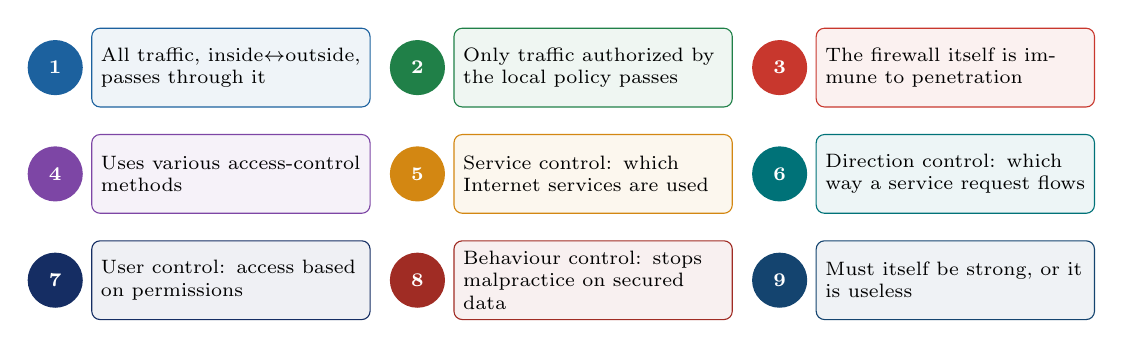
\begin{tikzpicture}
    \foreach \t/\c [count=\i from 0] in {
      All traffic\comma{} inside$\leftrightarrow$outside\comma{} passes through it/ocean,
      Only traffic authorized by the local policy passes/leaf!80!black,
      The firewall itself is immune to penetration/brick,
      Uses various access-control methods/grape,
      Service control: which Internet services are used/amber!90!black,
      Direction control: which way a service request flows/aqua!80!black,
      User control: access based on permissions/navy,
      Behaviour control: stops malpractice on secured data/brick!80!black,
      Must itself be strong\comma{} or it is useless/ocean!70!black}
    {
      \pgfmathsetmacro{\x}{mod(\i,3)*4.6}
      \pgfmathsetmacro{\y}{-floor(\i/3)*1.35}
      \node[circle,fill=\c,text=white,font=\scriptsize\bfseries,minimum size=7mm] (n\i) at (\x-1.85,\y) {\the\numexpr\i+1\relax};
      \node[draw=\c,fill=\c!7,rounded corners=3pt,anchor=west,text width=33mm,minimum height=10mm,font=\scriptsize] at ([xshift=1mm]n\i.east) {\t};
    }
  \end{tikzpicture}
  \vspace{3mm}

  {\small Inbound data is checked to be from an \textbf{authenticated user}; outbound data is checked to be going to an \textbf{authenticated person}.}
\end{frame}

% ------------------------------------------------------------
\begin{frame}{When a Firewall Hurts}
  \begin{columns}[c]
    \begin{column}{0.5\textwidth}
      \centering
      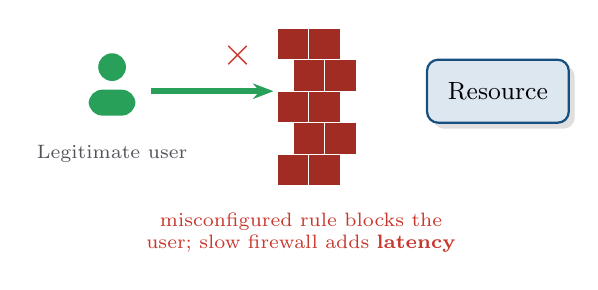
\begin{tikzpicture}
        \pic[scale=1.1] at (0,0) {person=leaf}; \node[tag] at (0,-0.6) {Legitimate user};
        \foreach \r in {0,...,4}{
          \pgfmathsetmacro{\off}{mod(\r,2)*0.2}
          \foreach \c in {0,1} \draw[white,fill=brick!80!black] (2.1+\off+\c*0.4,\r*0.4-1) rectangle ++(0.4,0.4);
        }
        \draw[flow=leaf,line width=2pt] (0.5,0.2) -- (2.05,0.2);
        \node[brick,font=\Large\bfseries] at (1.6,0.65) {$\times$};
        \node[box=ocean,minimum width=18mm] at (4.9,0.2) {Resource};
        \node[font=\scriptsize,text=brick,text width=40mm,align=center] at (2.4,-1.6) {misconfigured rule blocks the user; slow firewall adds \textbf{latency}};
      \end{tikzpicture}
    \end{column}
    \begin{column}{0.48\textwidth}
      \begin{alertblock}{Negative impacts}
        \small
        \begin{itemize}\setlength{\itemsep}{2pt}
          \item \textbf{Improper configuration} blocks access to desired resources
          \item An ordinary \textbf{multi-homed PC} used as a firewall may be too slow, causing \textbf{latency}
        \end{itemize}
      \end{alertblock}
      \vspace{2mm}
      \begin{block}{Two general methods}
        \small Most firewalls are variations of \textbf{packet filtering} or \textbf{proxy servers (application gateways)}.
      \end{block}
    \end{column}
  \end{columns}
\end{frame}

% ------------------------------------------------------------
\begin{frame}{Encryption in the Security System}
  \centering
  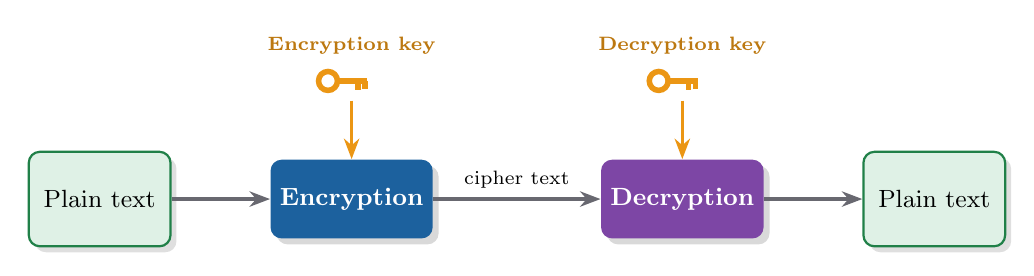
\begin{tikzpicture}
    \node[box=leaf,minimum width=18mm,minimum height=12mm] (p1) at (0,0) {Plain text};
    \node[solid box=ocean,minimum width=20mm,minimum height=10mm] (e) at (3.2,0) {Encryption};
    \node[solid box=grape,minimum width=20mm,minimum height=10mm] (d) at (7.4,0) {Decryption};
    \node[box=leaf,minimum width=18mm,minimum height=12mm] (p2) at (10.6,0) {Plain text};
    \draw[flow] (p1) -- (e); \draw[flow] (e) -- node[above,font=\scriptsize]{cipher text} (d); \draw[flow] (d) -- (p2);
    \pic at (2.9,1.5) {key=amber}; \node[font=\scriptsize\bfseries,text=amber!80!black] at (3.2,1.95) {Encryption key};
    \pic at (7.1,1.5) {key=amber}; \node[font=\scriptsize\bfseries,text=amber!80!black] at (7.4,1.95) {Decryption key};
    \draw[amber,very thick,->] (3.2,1.25) -- (e); \draw[amber,very thick,->] (7.4,1.25) -- (d);
  \end{tikzpicture}
  \vspace{3mm}
  \begin{columns}[T]
    \begin{column}{0.49\textwidth}
      \begin{block}{Why encryption matters}
        \small
        \textbullet~\textbf{Central} to all security mechanisms\\
        \textbullet~Gives \textbf{confidentiality} of data\\
        \textbullet~Some protocols rely on it for \textbf{availability}
      \end{block}
    \end{column}
    \begin{column}{0.49\textwidth}
      \begin{alertblock}{The cost}
        \small Encrypted data is \textbf{bigger}, so it needs more \textbf{bandwidth}, and devices need extra power to encrypt and decrypt.
      \end{alertblock}
    \end{column}
  \end{columns}
\end{frame}

% ------------------------------------------------------------
\begin{frame}{Intrusion Detection System (IDS)}
  \centering
  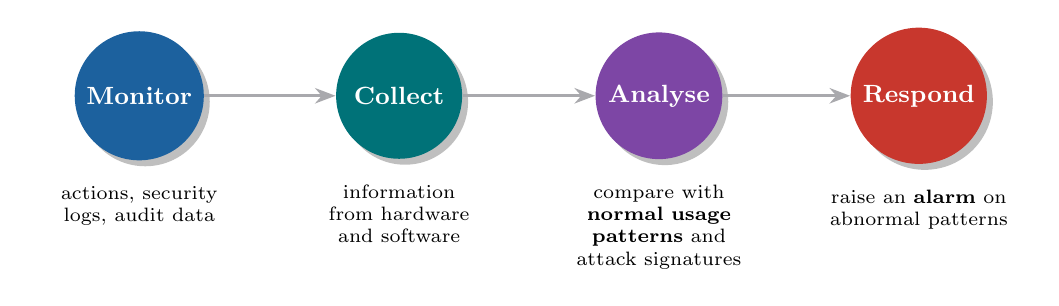
\begin{tikzpicture}
    \foreach \t/\c [count=\i from 0] in {Monitor/ocean,Collect/aqua!80!black,Analyse/grape,Respond/brick}{
      \node[circle,fill=\c,text=white,font=\small\bfseries,minimum size=16mm,drop shadow] (s\i) at (\i*3.3,0) {\t};
    }
    \foreach \i [evaluate=\i as \j using int(\i+1)] in {0,1,2} \draw[flow=ink!40] (s\i) -- (s\j);
    \node[font=\scriptsize,text width=26mm,align=center,below=2mm of s0] {actions, security logs, audit data};
    \node[font=\scriptsize,text width=26mm,align=center,below=2mm of s1] {information from hardware and software};
    \node[font=\scriptsize,text width=26mm,align=center,below=2mm of s2] {compare with \textbf{normal usage patterns} and attack signatures};
    \node[font=\scriptsize,text width=26mm,align=center,below=2mm of s3] {raise an \textbf{alarm} on abnormal patterns};
  \end{tikzpicture}
  \vspace{2mm}
  \begin{columns}[T]
    \begin{column}{0.49\textwidth}
      \begin{block}{What an IDS is}
        \small A combination of \textbf{hardware and software} that monitors and analyses activity to \textbf{detect attacks or intrusions}. Some respond automatically; some use scanners for vulnerability analysis.
      \end{block}
    \end{column}
    \begin{column}{0.49\textwidth}
      \begin{alertblock}{What an IDS cannot do}
        \small It \textbf{cannot stop crime}. It can only help prevent it and \textbf{provide evidence} for investigation.
      \end{alertblock}
    \end{column}
  \end{columns}
\end{frame}

% ------------------------------------------------------------
\begin{frame}{Software, Hardware and Policy Controls}
  \centering
  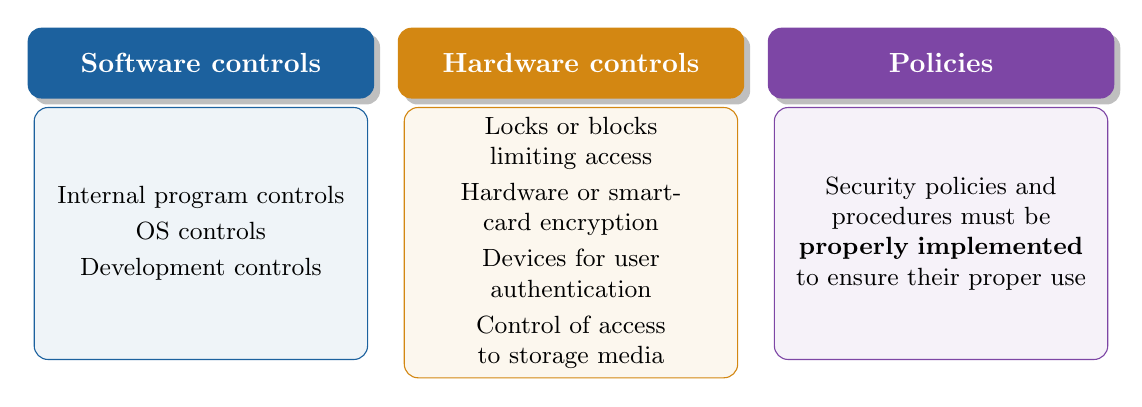
\begin{tikzpicture}
    \foreach \x/\c/\t/\d in {
      0/ocean/Software controls/{Internal program controls\\[2pt] OS controls\\[2pt] Development controls},
      4.7/amber!90!black/Hardware controls/{Locks or blocks limiting access\\[2pt] Hardware or smart-card encryption\\[2pt] Devices for user authentication\\[2pt] Control of access to storage media},
      9.4/grape/Policies/{Security policies and procedures must be \textbf{properly implemented} to ensure their proper use}}
    {
      \node[fill=\c,text=white,rounded corners=5pt,font=\bfseries,minimum width=44mm,minimum height=9mm,drop shadow] (h) at (\x,0) {\t};
      \node[draw=\c,fill=\c!7,rounded corners=5pt,text width=40mm,minimum height=32mm,font=\small,anchor=north,align=center] at ([yshift=-1mm]h.south) {\d};
    }
  \end{tikzpicture}
\end{frame}

% ------------------------------------------------------------
\begin{frame}{Physical Controls}
  \begin{columns}[c]
    \begin{column}{0.5\textwidth}
      \centering
      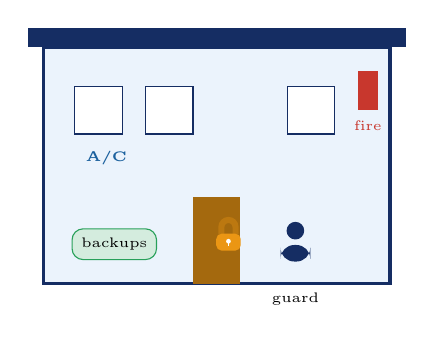
\begin{tikzpicture}
        % building
        \fill[sky,draw=navy,very thick] (0,0) rectangle (4.4,3.0);
        \fill[navy] (-0.2,3.0) rectangle (4.6,3.25);
        \fill[amber!70!black] (1.9,0) rectangle (2.5,1.1);
        \pic[scale=0.6] at (2.35,0.55) {lock=amber};
        \pic[scale=0.7] at (3.2,0.35) {person=navy}; \node[font=\tiny] at (3.2,-0.2) {guard};
        \foreach \x in {0.4,1.3,3.1} \fill[white,draw=navy] (\x,1.9) rectangle ++(0.6,0.6);
        \node[font=\tiny\bfseries,text=ocean] at (0.8,1.6) {A/C};
        \fill[brick] (4.0,2.2) rectangle (4.25,2.7); \node[font=\tiny,text=brick] at (4.12,2.0) {fire};
        \node[fill=leaf!20,draw=leaf,font=\tiny,rounded corners] at (0.9,0.5) {backups};
      \end{tikzpicture}
    \end{column}
    \begin{column}{0.48\textwidth}
      \begin{block}{Easy to implement, effective and less costly}
        \small
        \begin{itemize}\setlength{\itemsep}{1pt}
          \item Locks on doors; \textbf{guards} at entry and exit points
          \item Backup copies of critical software and data
          \item Access control and media control
          \item Precautions against \textbf{water and fire} damage
          \item Air conditioning
          \item Site planning that minimizes \textbf{natural disaster} risk
        \end{itemize}
      \end{block}
    \end{column}
  \end{columns}
\end{frame}

% ------------------------------------------------------------
\begin{frame}{System Security and Virus Controls}
  \begin{columns}[T]
    \begin{column}{0.44\textwidth}
      \begin{block}{System security}
        \small \textbf{International security standards}: most vendors now build their security facilities to these standards.
      \end{block}
      \centering
      
\begin{tikzpicture}
        \node[circle,fill=ocean,text=white,font=\scriptsize\bfseries,minimum size=17mm,align=center,drop shadow] {Standards\\built in};
      \end{tikzpicture}
    \end{column}
    \begin{column}{0.54\textwidth}
      \begin{alertblock}{Computer virus controls}
        \small
        \begin{itemize}\setlength{\itemsep}{2pt}
          \item Keep \textbf{updated} virus protection and detection software
          \item Scan \textbf{internal and external} drives regularly
          \item Screen all diskettes and software with a virus scanner \textbf{before loading}
        \end{itemize}
      \end{alertblock}
      \centering
      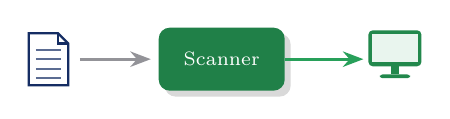
\begin{tikzpicture}
        \pic at (0,0) {doc=navy};
        \draw[flow=ink!50] (0.4,0) -- (1.3,0);
        \node[solid box=leaf!80!black,minimum width=16mm,font=\scriptsize] (sc) at (2.2,0) {Scanner};
        \draw[flow=leaf] (sc) -- (4.0,0);
        \pic[scale=0.8] at (4.4,-0.05) {pc=leaf};
      \end{tikzpicture}
    \end{column}
  \end{columns}
\end{frame}

% ------------------------------------------------------------
\begin{frame}{Personnel Security}
  \centering
  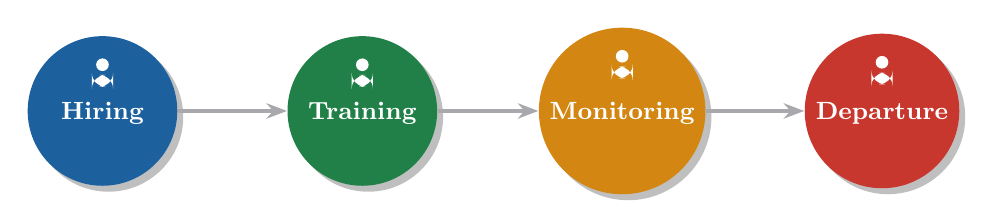
\begin{tikzpicture}
    \foreach \t/\c [count=\i from 0] in {Hiring/ocean,Training/leaf!80!black,Monitoring/amber!90!black,Departure/brick}{
      \node[circle,fill=\c,text=white,font=\small\bfseries,minimum size=19mm,text depth=-3mm,drop shadow] (s\i) at (\i*3.3,0) {\t};
      \pic[scale=0.5] at ([yshift=-6mm]s\i.north) {person=white};
    }
    \foreach \i [evaluate=\i as \j using int(\i+1)] in {0,1,2} \draw[flow=ink!40] (s\i) -- (s\j);
  \end{tikzpicture}
  \vspace{3mm}
  \begin{columns}[c]
    \begin{column}{0.55\textwidth}
      \begin{block}{Definition}
        \small Everything involving \textbf{employees}, who are potential elements of security breaches: hiring, training, monitoring them, and handling their departure.
      \end{block}
    \end{column}
    \begin{column}{0.42\textwidth}
      \centering
      \begin{tikzpicture}
        \fill[ink!10] (0,0) circle (1.0);
        \fill[brick] (0,0) -- (90:1.0) arc (90:-198:1.0) -- cycle;
        \node[white,font=\small\bfseries] at (-54:0.5) {80\%+};
        \node[font=\scriptsize,text width=30mm,anchor=west] at (1.15,0) {of incidents are due to \textbf{internal users}};
      \end{tikzpicture}
    \end{column}
  \end{columns}
  \vspace{1mm}

  {\small Most breaches are caused by \textbf{people}, and the most common perpetrators are the \textbf{legitimate users} of the system.}
\end{frame}

% ------------------------------------------------------------
\begin{frame}{Auditing}
  \begin{columns}[c]
    \begin{column}{0.5\textwidth}
      \centering
      \begin{tikzpicture}
        \node[draw=navy,thick,fill=white,minimum width=56mm,minimum height=38mm,rounded corners=3pt,drop shadow] (log) at (0,0) {};
        \node[fill=navy,text=white,font=\scriptsize\bfseries,minimum width=56mm,anchor=north] at (log.north) {security.log};
        \foreach \t/\c [count=\i from 0] in {09:02 ravi login OK/ink!70,09:15 sita login OK/ink!70,02:11 admin login FAIL/brick,02:11 admin login FAIL/brick,02:12 admin login FAIL/brick,02:14 ravi login from 3 places/brick,03:00 shutdown db-server/brick}
          \node[anchor=west,font=\tiny\ttfamily,text=\c] at (-2.65,1.15-\i*0.38) {\t};
        \draw[brick,very thick,rounded corners] (-2.75,0.58) rectangle (2.75,-1.55);
        \node[fill=brick,text=white,font=\tiny\bfseries,rounded corners] at (2.2,-1.75) {RED FLAGS};
      \end{tikzpicture}
    \end{column}
    \begin{column}{0.48\textwidth}
      \begin{itemize}\small\setlength{\itemsep}{3pt}
        \item A \textbf{tedious} process that needs a good eye for detail
        \item Track everyone who \textbf{logs on and off}
        \item Audit movement of \textbf{critical files}, attempted deletions, and access to mission-critical data
      \end{itemize}
      \begin{alertblock}{Red flags}
        \scriptsize Multiple bad log-on attempts \,$\cdot$\, one account logging in from many places at once \,$\cdot$\, attempted shutdown of critical servers
      \end{alertblock}
      {\scriptsize An organization that skips its logs may be \textbf{unable to tell the legal agencies} that an incident really happened.}
    \end{column}
  \end{columns}
\end{frame}

% ------------------------------------------------------------
\begin{frame}{Putting It Together: The Multi-Level Model}
  \begin{columns}[c]
    \begin{column}{0.52\textwidth}
      \centering
      \begin{tikzpicture}
        \foreach \r/\c/\t in {3.0/navy/Policies \& auditing,2.45/brick/Personnel security,1.9/amber!90!black/Physical controls,1.35/ocean/Firewall \& IDS,0.8/grape/Access control \& passwords}{
          \fill[\c!85] (0,0) circle (\r);
          \node[white,font=\tiny\bfseries] at (0,\r-0.27) {\t};
        }
        \fill[leaf] (0,0) circle (0.52);
        \node[white,font=\scriptsize\bfseries,align=center] at (0,0) {Data};
      \end{tikzpicture}
    \end{column}
    \begin{column}{0.46\textwidth}
      \begin{block}{Defence in depth}
        \small No single control is perfect. Security works in \textbf{layers}: if an attacker gets past one, the next one is still there.
      \end{block}
      \vspace{2mm}
      \begin{itemize}\small\setlength{\itemsep}{3pt}
        \item Lesson 4 decides \textbf{what} to protect and \textbf{why}
        \item Lesson 7 gives the \textbf{facilities} to protect it at every level
      \end{itemize}
    \end{column}
  \end{columns}
\end{frame}

% ------------------------------------------------------------
\begin{frame}{Module 3 Summary}
  \begin{columns}[T]
    \begin{column}{0.49\textwidth}
      \begin{block}{Lesson 4: Security and Authorization}
        \small
        \begin{itemize}\setlength{\itemsep}{0pt}
          \item Goals: integrity, confidentiality, availability
          \item Risk analysis: assets, threats, impact
          \item Threats, vulnerabilities and controls
          \item Method, opportunity, motive
          \item Know, have, are; MAC vs.\ DAC; tokens
        \end{itemize}
      \end{block}
    \end{column}
    \begin{column}{0.49\textwidth}
      \begin{exampleblock}{Lesson 7: Multi Level Model of Security}
        \small
        \begin{itemize}\setlength{\itemsep}{0pt}
          \item Access, password and account management
          \item Data, resource and sensitive system protection
          \item Backups, firewalls, encryption, IDS
          \item Software, hardware and physical controls
          \item Personnel security and auditing
        \end{itemize}
      \end{exampleblock}
    \end{column}
  \end{columns}
  \vspace{1mm}
  \begin{alertblock}{Review questions}
    \scriptsize
    1.~Discuss the goals of computer security. \quad 2.~What are the security problems and requirements? \quad
    3.~Explain threats and vulnerabilities. \quad 4.~Write a short note on user authentication. \quad
    5.~Explain security systems and facilities in network security.
  \end{alertblock}
\end{frame}

% ------------------------------------------------------------
\begin{frame}{References}
  \begin{enumerate}\setlength{\itemsep}{8pt}
    \item William Stallings, \emph{Cryptography and Network Security}, PHI Publishers.
    \item Charlie Kaufman, Radia Perlman, \emph{Network Security}, Pearson Education.
    \item Bruce Schneier, \emph{Applied Cryptography}, John Wiley \& Sons.
    \item Roberta Bragg, \emph{Network Security: The Complete Reference}, TMH.
  \end{enumerate}
  \vspace{6mm}
  \centering
  \begin{tikzpicture}
    \node[fill=navy,text=white,rounded corners=8pt,inner sep=10pt,font=\Large\bfseries,drop shadow] {Thank You! \; Questions?};
  \end{tikzpicture}
\end{frame}

\end{document}
